\newpage

\section{Die neuronalen Netze}\label{die neuronalen netze}

Die Regenvorhersage mit Hilfe von künstlichen neuronalen Netzen (KNN) möchten wir mit einem Zitat einführen.
Der Nobelpreisträge Richard P. Feynman ist in einem Gespräch mit einem nicht namentlich erwähnten Laien wobei es um die Existenz fliegender Untertassen geht. Feynman trifft die Aussage, dass es sehr unwahrscheinlich ist, dass es fliegende Untertassen gibt. Der Laie antwortet darauf, dass das sehr unwissenschaftlich sei, worauf Feynman erwiedert:

\begin{quote}{Richard P. Feynman}
''...But that is the way that is scientific. It is scientific only to say what is more likely and what less likely, and not to be proving all the time the possible and impossible.''  
\end{quote}

\noindent Treffend wird in dem Gespräch von Feynman erläutert, dass der wissenschaftliche Weg eine Wahrscheinlichkeit beinhaltet, die Auskunft über das Eintreten eines Ereignisses gibt. Wir werden für die Regenvorhersage also eine probabilistische Aussage treffen. Dies bedeutet insbesondere, dass eine Verteilung für die Regenvorhersage geschätzt wird, durch die eine Aussage über die Regenwahrscheinlichkeit und auch die Wahrscheinlichkeit der Intensität getroffen werden kann.\\

\noindent Bei der Regenvorhersage via KNN bekommt das KNN als Input ein Set von Bildern, woraus ein Feld von Parametern geschätzt wird, wodurch in Kombination mit der zugehörigen Verteilung eine 30-minütige Vorhersage generiert werden kann. Dieser Vorgang ist in der nachfolgenden Abbildung skizziert.


\begin{figure}[htb]
 \centering
 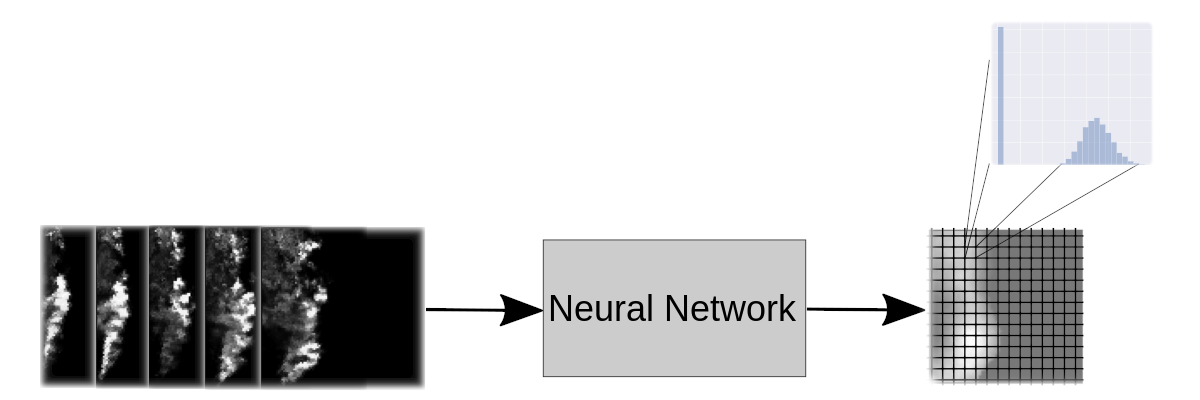
\includegraphics[width=1.0\textwidth,angle=0]{abb/skizzierung_regenvorhersage}
 \caption{Skizzierung der Vorhersage}
\label{fig:Vorhersage_skizze}
\end{figure}

\noindent Wie aus Abbildung \ref{fig:Vorhersage_skizze} hervorgeht, besteht der Ausgang des KNN aus einem Feld von Verteilungen. Diese Verteilungen nehmen wir als unabhängig an.
Die zu schätzende Verteilung ist im vornherein nicht klar, weshalb wir eingangs drei Verteilungen begutachten.
Wir schauen uns die Multinomiale, und die negativ Binomial Verteilung an.
Die negativ Binomialverteilung wird allerdings mit der Multinomialen Verteilung gemischt, sodass wir die ''Zero Inflated negativ Binomial'' Verteilung (ZINB) erhalten.
Dies kann so aufgefasst werden, dass wir eine Bernoulli-Verteilung für die binäre Entscheidung über Regen oder kein Regen erhalten. Für den Fall dass Regen vorhergesagt wird, greifen wir auf die Negativ Binomialverteilung zurück.
\\

\subsection{Netzwerk Topologie}

\noindent Wir schauen uns zwei verschiedene Netzwerarchitekturen an. Hierbei passen wir uns den Beschränkungen der uns zur Verfügung stehenden Hardware an.
Uns steht eine Geforce 2060 Super mit 8GB VRAM zur Verfügung. Die Netzwertopologie ist auf die Größe des VRAMS beschränkt, wir werden unser Netzwerk also auf diese Größe beschränken. Die Größe der Eingangsbilder setzen wir auf 96x96 Pixel fest und die Größe der Ausgangsbilder auf 64x64. Die Patches werden um den Pixel, der Konstanz repräsentiert ausgeschnitten.
Alle Netzwerke die wir trainieren haben die Klassifikationsschicht gemeinsam, unterscheiden sich jedoch für die verschiedenen Verteilungen.\\

\begin{figure}[h]
 \centering
\begin{tikzpicture}[inputnode/.style={circle, draw=black!60, fill=green!5,  minimum size=10mm},
input/.style={circle},
outputnode/.style={circle},
]


\node[rectangle, 
dashed, 
draw=sublimedg, 
fill=gray,  
fill opacity=0.2,
very thick, 
minimum width=40em, 
minimum height=20.0em] (duh) at (4, 3) {};

\node[input]            (x0)               at (-3,3)         {};

\node[inputnode]        (inputlayer)       at (3,2)         {};
\node[input]            (x4)               at (3,3)         {$\vdots$};
\node[input]            (x2_3)             at (3.5,3)       {256};
\node[inputnode]        (inputlayer_1)     at (3,4)         {};

\node[outputnode]       (outputlayer)      at (6,2)         {};
\node[inputnode]        (x1)               at (0,5)         {};
\node[input]            (x2)               at (0,3)         {$\vdots$};
\node[input]            (x2_2)             at (0,3.5)       {4096};
\node[inputnode]        (x3)           	   at (0,1)         {};


\node[inputnode]        (x5)               at (6,5)         {};
\node[input]            (x6)               at (6,3)         {$\vdots$};
\node[input]            (x2_1)             at (6,3.5)       {4096 x $n$};
\node[inputnode]        (x7)           	   at (6,1)         {};
%\node[inputnode]        (x9)           	   at (10,3)         {};

\node[cascaded,
		minimum width=4em, 
		minimum height=4em] (x9) at (10,3) {64x64};

\draw[-latex] (x1.east) -- node[above] {} (inputlayer.west);
\draw[-latex] (x3.east) -- node[above] {} (inputlayer.west);
\draw[-latex] (x1.east) -- node[above] {} (inputlayer_1.west);
\draw[-latex] (x3.east) -- node[above] {} (inputlayer_1.west);

\draw[-latex] (inputlayer.east) -- node[above] {} (x5.west);
\draw[-latex] (inputlayer.east) -- node[above] {} (x7.west);

\draw[-latex] (inputlayer_1.east) -- node[above] {} (x5.west);
\draw[-latex] (inputlayer_1.east) -- node[above] {} (x7.west);

\draw[-latex] (x0.east) -- node[above] {Flatten} (x2.west);
\draw[-latex] (x6.east) -- node[above] {64x64x$n$} (x9.west);

\end{tikzpicture}
 \caption{Klassifikationsschicht, $n$ variiert hierbei je nach Verteilung. Für die Zero-Inflated Poisson Verteilung ist $n$ gleich 2, für die Zero-Inflated Negativ Binomial Verteilung ist $n$ gleich 3, und für die Multinomiale Verteilung ist $n$ gleich 7  }
\label{fig:classification_layer}
\end{figure}

\newpage
\noindent Wir verwenden zum einen die Unet-Architektur, wie sie von unseren Vorgängern verwendet wird. Diese Architektur ist in der folgenden Abbildung zu sehen.



\begin{figure}[h]
 \centering
\begin{tikzpicture}[thick,scale=0.5, every node/.style={scale=0.5},inputnode/.style={circle, draw=black!60, fill=green!5,  minimum size=10mm},
input/.style={circle},
outputnode/.style={circle},]
	

	% Schicht 1
	\node[input,rotate=90] (top1_txt) at (0.5,-1) {64x64};
	\node[slimconv] (top1) at (1, 1) {5} ;
	\node[slimconv] (top2) at (2.0, 1) {20} ;
	\node[slimconv] (top3) at (3.0, 1) {20};
	\draw[-stealth, very thick] (top1.east) -- (top2);
	\draw[-stealth, very thick] (top2.east) -- (top3);


	% Schicht 2
	\node[input,rotate=90] (top1_txt) at (2.5,-4.25) {32x32};
	\node[slimconv,
			minimum height=6em] (top1_1) at (3.0, -3.5) {25};
	\node[slimconv,
			minimum width=1.5em, 
			minimum height=6em] (top2_1) at (4.0, -3.5) {25};
	\node[slimconv,
			minimum width=1.5em, 
			minimum height=6em] (top3_1) at (5.125, -3.5) {25};
	\draw[-stealth, very thick] (top1_1.east) -- (top2_1);
	\draw[-stealth, very thick] (top2_1.east) -- (top3_1);
	\draw[-stealth, very thick,red] (top3.south) -- (top1_1.north);


	% Schicht 3
	\node[input,rotate=90] (top1_txt) at (4.5,-6.125) {16x16};
	\node[slimconv,
			minimum width=2em, 
			minimum height=3em] (top1_2) at (5.125, -6.0) {25};
	\node[slimconv,
			minimum width=2.5em, 
			minimum height=3em] (top2_2) at (6.75, -6.0) {25};
	\node[slimconv,
			minimum width=2.5em, 
			minimum height=3em] (top3_2) at (8.5, -6.0) {25};

	\draw[-stealth, very thick] (top1_2.east) -- (top2_2);
	\draw[-stealth, very thick] (top2_2.east) -- (top3_2);
	\draw[-stealth, very thick,red] (top3_1.south) -- (top1_2.north);


	% Schicht 4
	\node[input,rotate=90] (top1_txt) at (7.825,-7.75) {8x8};
	\node[slimconv,
			minimum width=2em, 
			minimum height=2em] (top1_3) at (8.5, -7.75) {25};
	\node[slimconv,
			minimum width=3.5em, 
			minimum height=2em] (top2_3) at (10.25, -7.75) {25};
	\node[slimconv,
			minimum width=3.5em, 
			minimum height=2em] (top3_3) at (12.25, -7.75) {25};

	\draw[-stealth, very thick] (top1_3.east) -- (top2_3);
	\draw[-stealth, very thick] (top2_3.east) -- (top3_3);
	\draw[-stealth, very thick,red] (top3_2.south) -- (top1_3.north);



	% Schicht 5
	\node[input,rotate=90] (top1_txt) at (11.25,-9.25) {4x4};
	\node[slimconv,
			minimum width=3.5em, 
			minimum height=1.5em] (top1_4) at (12.25, -9.25) {25};
	\node[slimconv,
			minimum width=3.5em, 
			minimum height=1.5em] (top3_4) at (16.75, -9.25) {25};

	%\draw[-stealth, very thick] (top1_4.east) -- (top3_4) ;
	\draw[-stealth, very thick] (top1_4.east) -- (top3_4);
	\draw[-stealth, very thick,red] (top3_3.south) -- (top1_4.north);

	% Schicht 4 ( UP )

	\node[slimconv,
			minimum width=2em,
			fill=white,
			minimum height=2em] (top4_30) at (15.6, -7.75) {};
	\node[slimconv,
			minimum width=3.5em, 
			minimum height=2em] (top4_31) at (16.75, -7.75) {50};
	\node[slimconv,
			minimum width=3.5em, 
			minimum height=2em] (top5_3) at (19.25, -7.75) {50};
	\node[slimconv,
			minimum width=3.5em, 
			minimum height=2em] (top6_3) at (21.25, -7.75) {50};


	
	\draw[-stealth, very thick,opacity=0.5] (top3_3.east) -- (top4_30.west);
	\draw[-stealth, very thick] (top4_31.east) -- (top5_3);
	\draw[-stealth, very thick] (top5_3.east) -- (top6_3);
	\draw[-stealth, very thick,green] (top3_4.north) -- (top4_31.south);


		% Schicht 3 (UP)
	\node[slimconv,
			minimum width=2em,
			fill=white,
			minimum height=3em] (top4_20) at (20.125, -6.0) {};
	\node[slimconv,
			minimum width=3.5em, 
			minimum height=3em] (top4_21) at (21.25, -6.0) {75};
	\node[slimconv,
			minimum width=2.5em, 
			minimum height=3em] (top5_2) at (23.25, -6.0) {75};
	\node[slimconv,
			minimum width=2.5em, 
			minimum height=3em] (top6_2) at (25, -6.0) {75};


	\draw[-stealth, very thick,opacity=0.5] (top3_2.east) -- (top4_20.west);
	\draw[-stealth, very thick] (top4_21.east) -- (top5_2);
	\draw[-stealth, very thick] (top5_2.east) -- (top6_2);
	\draw[-stealth, very thick,green] (top6_3.north) -- (top4_21.south);

	% Schicht 2
	\node[slimconv,
		minimum width=1.5em,
		fill=white,
		minimum height=6em] (top4_10) at (24.18, -3.5) {};
	\node[slimconv,
			minimum width=2.5em,
			minimum height=6em] (top4_11) at (25.0, -3.5) {100};
	\node[slimconv,
			minimum width=1.5em, 
			minimum height=6em] (top5_1) at (26.5, -3.5) {100};
	\node[slimconv,
			minimum width=1.5em, 
			minimum height=6em] (top6_1) at (27.75, -3.5) {100};

	\draw[-stealth, very thick,opacity=0.5] (top3_1.east) -- (top4_10.west);
	\draw[-stealth, very thick] (top4_11.east) -- (top5_1);
	\draw[-stealth, very thick] (top5_1.east) -- (top6_1);
	\draw[-stealth, very thick,green] (top6_2.north) -- (top4_11.south);



	
	\node[slimconv,fill=white,] (top4_0) at (27.125, 1) {};
	\node[slimconv] (top4_1) at (27.75, 1) {120};
	\node[slimconv] (top5) at (29, 1) {n};
%	\node[slimconv] (top6) at (29.75, 1) {};

	\draw[-stealth, very thick,opacity=0.5] (top3.east) -- (top4_0.west);
	\draw[-stealth, very thick] (top4_1.east) -- (top5);
%	\draw[-stealth, very thick] (top5.east) -- (top6);
	\draw[-stealth, very thick,green] (top6_1.north) -- (top4_1.south);





	\node[input]        (A1)       at (27.75, -8)         {};
	\node[input]        (A2)       at (27.75, -9.5)         {};
	\draw[-stealth, very thick,green] (A2.north) -- node[right,opacity=1.0,black] {Up-Sampling} (A1.south);


	\node[input]        (A3)       at (27.75, -6)         {};
	\node[input]        (A4)       at (27.75, -7.5)         {};
	\draw[-stealth, very thick,red] (A3.south) -- node[right,opacity=1.0,black] {Pooling} (A4.north);



	\node[input]        (A5)       at (27.75, -7.75)         {};
	\node[input]        (A6)       at (30.0, -7.75)         {Conv 3x3};
	\draw[-stealth, very thick,black] (A5.east) -- (A6.west);



	\node[input]        (A7)       at (25.75, -7.75)         {};
	\node[input]        (A8)       at (27.25, -7.75)         {};
	\draw[-stealth, very thick,gray] (A7.east) --node[above,opacity=1.0,black]{Skipping} (A8.west);


\node[rectangle, 
dashed, 
draw=sublimedg, 
fill=gray,  
fill opacity=0.4,
very thick, 
minimum width=5em, 
minimum height=5em] (kl) at (31, 1) {Kl-Schicht};
	\draw[-stealth, very thick] (top5.east) -- (kl.west);

\end{tikzpicture}
 \caption{Abgespekte Version des Unets  
}\label{fig:Unet1}
\end{figure}

\noindent Die abgespekte Version des Unets hat im Gegensatz zur originalen Architektur wesentlich weniger Gewichte.
Hier sind es ca 10 000 trainierbare Gewichte. Zusätzliche Gewichte liegen in der Klassifikationsschicht (Kl-Schicht in Bild \ref{fig:classification_layer}).\\


\noindent Eine weitere Architektur die wir begutachten ist ein Mix aus Inception-Layer und CNN-LSTM-Layer. Die Regenvorhersage in unserem Setup wird für gewöhnlich auch als Next-Frame prediction bezeichnet. Aus einem Set aufeinanderfolgender Eingangsbilder wird eine plausible Vorhersage für das nächste Bild erzeugt.


%\begin{wrapfigure}{R}{0.5\textwidth}
\begin{figure}[h]
 \centering
\begin{tikzpicture}[thick,scale=0.8, every node/.style={scale=0.8}]

\node[rectangle, 
dashed, 
draw=sublimedg, 
fill=gray,  
fill opacity=0.2,
very thick, 
minimum width=20em, 
minimum height=21.0em] (duh) at (2.75, -7.25) {};


\node[cascaded,
		minimum width=4em, 
		minimum height=4em] (conv1) at (1, -10) {1x1};

\node[cascaded,
		minimum width=4em, 
		minimum height=4em] (conv3x3) at (3, -10) {3x3};

\node[cascaded,
		minimum width=4em, 
		minimum height=4em] (conv3x3_1) at (5, -10) {3x3};

\node[cascaded,
		minimum width=4em, 
		minimum height=4em] (conv3x3_2) at (4.5, -7.5) {3x3};


\node[cascaded,
		minimum width=4em, 
		minimum height=4em] (conv3x3_2) at (3, -5.0) {stack};

%\draw[very thick, sublimedg, dashed] 

\node[rectangle, dashed, draw=sublimedg, fill=white,  fill opacity=0.5,very thick, minimum width=1.0em, minimum height=1.0em] (R0) at (1.5, -9.5) {};

\node[rectangle, dashed, draw=sublimedg, fill=white,  fill opacity=0.5,very thick, minimum width=1.0em, minimum height=1.0em] (R1) at (3.5, -9.5) {};

\node[rectangle, dashed, draw=sublimedg, fill=white,  fill opacity=0.5,very thick, minimum width=1.0em, minimum height=1.0em] (R2) at (5.5, -9.5) {};

\node[rectangle, dashed, draw=sublimedg, fill=white,  fill opacity=0.5,very thick, minimum width=1.0em, minimum height=1.0em] (R3) at (5.0, -7.0) {};


\node[circle, inner sep = 0.1em, fill=sublimedg] (C0) at (2.5, -5.5) {};
\node[circle, inner sep = 0.1em, fill=sublimedg] (C1) at (2.75, -5.5) {};
\node[circle, inner sep = 0.1em, fill=sublimedg] (C2) at (5, -8.0) {};
\node[circle, inner sep = 0.1em, fill=sublimedg] (C3) at (3, -5.5) {};



\draw[very thick, sublimedg, dashed] (R0.north east) -- (C0);
\draw[very thick, sublimedg, dashed] (R0.north west) -- (C0);
\draw[very thick, sublimedg, dashed] (R0.south west) -- (C0);
\draw[very thick, sublimedg, dashed] (R0.south east) -- (C0);

\draw[very thick, sublimedg, dashed] (R1.north east) -- (C1);
\draw[very thick, sublimedg, dashed] (R1.north west) -- (C1);
\draw[very thick, sublimedg, dashed] (R1.south west) -- (C1);
\draw[very thick, sublimedg, dashed] (R1.south east) -- (C1);


\draw[very thick, sublimedg, dashed] (R2.north east) -- (C2);
\draw[very thick, sublimedg, dashed] (R2.north west) -- (C2);
\draw[very thick, sublimedg, dashed] (R2.south west) -- (C2);
\draw[very thick, sublimedg, dashed] (R2.south east) -- (C2);

\draw[very thick, sublimedg, dashed] (R3.north east) -- (C3);
\draw[very thick, sublimedg, dashed] (R3.north west) -- (C3);
\draw[very thick, sublimedg, dashed] (R3.south west) -- (C3);
\draw[very thick, sublimedg, dashed] (R3.south east) -- (C3);





%\draw[very thick, sublimedg, dashed] (R1C.north east) -- (C1C);
\end{tikzpicture}
 \caption{Aufbau der von uns verwendeten Inception Layer, angelehnt an die inception Layer im Paper }
\label{fig:inception v2}
\end{figure}

\newpage

\noindent In der nachfolgenden Abbildung ist die von uns verwendete Architektur zu sehen. Diese Architektur ist angelehnt an die Inception-LSTM Layer des Papers ''Inception-inspired LSTM for Next-frame Video Prediction'' von \cite{hosseini2019inceptioninspired}. Wie Eingangs erwähnt beschränkt die Hardware (und auch die größe der Bilder) unsere Architektur und aus diesem Grund werden nicht mehr LSTM-Layer gestackt, wie im Paper beschrieben.
\begin{figure}[h]
 \centering
\begin{tikzpicture}[thick,scale=0.8, every node/.style={scale=0.8},->,>=stealth',shorten >=1pt,auto,node distance=2cm,
  thick,main node/.style={circle,fill=blue!30,draw,
  font=\sffamily\Large\bfseries,minimum size=15mm}]



\node[rectangle, 
dashed, 
draw=sublimedg, 
fill=gray,  
fill opacity=0.4,
very thick, 
minimum width=5em, 
minimum height=5em] (inc1) at (1, 1) {Inception Layer};
	

\node[main node,font=\sffamily\small] (LSTM_1) at (6,1) {CNN-LSTM}
  (LSTM_1) edge [loop right] (LSTM_1);

\node[main node,font=\sffamily\small] (LSTM_2) at (6,-2.5) {CNN-LSTM}
  (LSTM_2) edge [loop right] (LSTM_2);

\node[main node,font=\sffamily\small] (LSTM_3) at (6,-6) {CNN-LSTM};
  

\draw[very thick, sublimedg] (LSTM_1.south) -- (LSTM_2.north);
\draw[very thick, sublimedg] (LSTM_2.south) -- (LSTM_3.north);

\draw[very thick, sublimedg] (inc1.east) -- (LSTM_1.west);




\node[rectangle, 
dashed, 
draw=sublimedg, 
fill=gray,  
fill opacity=0.4,
very thick, 
minimum width=5em, 
minimum height=5em] (inc2) at (1, -2.5) {Inception Layer};



\node[rectangle, 
dashed, 
draw=sublimedg, 
fill=gray,  
fill opacity=0.4,
very thick, 
minimum width=5em, 
minimum height=5em] (inc3) at (1, -6) {Inception Layer};


\node[rectangle, 
dashed, 
draw=sublimedg, 
fill=gray,  
fill opacity=0.4,
very thick, 
minimum width=5em, 
minimum height=5em] (inc4) at (1, -9.5) {Inception Layer};



\node[rectangle, 
dashed, 
draw=sublimedg, 
fill=gray,  
fill opacity=0.4,
very thick, 
minimum width=5em, 
minimum height=5em] (inc5) at (3, -13) {Inception Layer};

\draw[very thick, sublimedg] (inc1.south) -- (inc2.north);
\draw[very thick, sublimedg] (inc2.south) -- (inc3.north);
\draw[very thick, sublimedg] (inc3.south) -- (inc4.north);
\draw[very thick, sublimedg] (inc4.south) -- (inc5.north);
\draw[very thick, sublimedg] (LSTM_3.south) -- (inc5.north);


\node[cascaded,
		minimum width=4em, 
		minimum height=4em] (conv1) at (6.5, -13) {7x7};


\node[cascaded,
		minimum width=4em, 
		minimum height=4em] (conv2) at (9.5, -13) {7x7};



\node[rectangle, 
dashed, 
draw=sublimedg, 
fill=gray,  
fill opacity=0.4,
very thick, 
minimum width=5em, 
minimum height=5em] (kl) at (12.5, -13) {Kl-Schicht};



\draw[very thick, sublimedg] (inc5.east) -- (conv1.west);
\draw[very thick, sublimedg] (conv1.east) -- (conv2.west);
\draw[very thick, sublimedg] (conv2.east) -- (kl.west);

\end{tikzpicture}
 \caption{LSTM Architektur}
\label{fig:LSTM-CNN}
\end{figure}

\noindent Unsere Architektur unterscheidet sich jedoch von der im Paper vorgestellten Architektur insofern, als dass die Inception-Layer nicht in das LSTM-Modul eingebaut sind.
Wir verwenden hierbei herkömmliche Convolution-LSTM Layer. Die Inception-Layer sind hierbei lediglich vor oder nach den Convolution-LSTM Layern zu finden.
Der Vorteil von Inception-Layer ist, dass diese in die Breite und nicht so sehr in die Tiefe gehen. Das hat zum Vorteil, dass beim aktualisieren der Gewichte der Gradient nicht so weit in das Netzwerk durchgereicht werden muss. Dadurch soll das Auftreten des vanishing Gradients vermindert werden und das aktualisieren der Gewichte bzw. das lernen verbessert werden.\\

\subsection{Training}
Beide Architekturen werden mindestens 35 Epochen trainiert, wobei die Architektur mit den LSTM-Layern 1:30 Stunden benötigt, das Unet hingegen benötigt ca. 10 Minuten pro Epoche.
Für das Training nutzen wir alle Daten der Jahre 2008 bis einschließlich 2017. Das entspricht insgesamt ca. 1 051 200 Zeitschritten. Hierbei werden 75\% der Daten für das Training und 25\% der Daten für das Testset verwendet.
Da der Hauptteil der Regendaten Null ist, also kein Regen vorhanden ist, liegt der Mittelwert der Daten schon nahe Null. Das bedeutet, dass der Mittelwert nicht (wie üblich) auf Null normiert wird.
Die Standardabweichung ist ebenfalls nahe Null, weshalb die Standardabweichung der Daten nicht auf Eins normieren (Dies würde zur Folge haben, dass Werte wesentlich größer als 1 sein können). 
Die Eingangsdaten werden allerdings auf den Bereich zwischen Null und Eins normiert.\\

\noindent Für den Ausgang der Netzwerke beschränkten wir uns auf einen 64x64 großen Pixelbereich, bei dem Konstanz in der Mitte liegt. Die Eingangsbilder bestehen aus einem 96x96 großen Pixelbereich um Konstanz. Regenfreie Bilder werden aussortiert, da diese Daten keinerlei Informationen beinhalten und das vorhandene Klassenungleichgewicht verstärken. Als Regularisierungsmaßnahme werden die Trainingsdaten pro Epoche um wenige Pixel verschoben, was zur Folge hat, dass das Netzwerk in jeder Epoche auf etwas unterschiedliche Daten trainiert. Als Kostenfunktion verwenden wir die Negative Loglikelihood.
\\

\noindent In der Nachfolgenden Abbildung sind die Trainingskurve für die beiden Architekturen zu sehen. Die hierfür Verwendete Verteilung ist die ZINB.

\begin{figure}[htb]
 \centering
 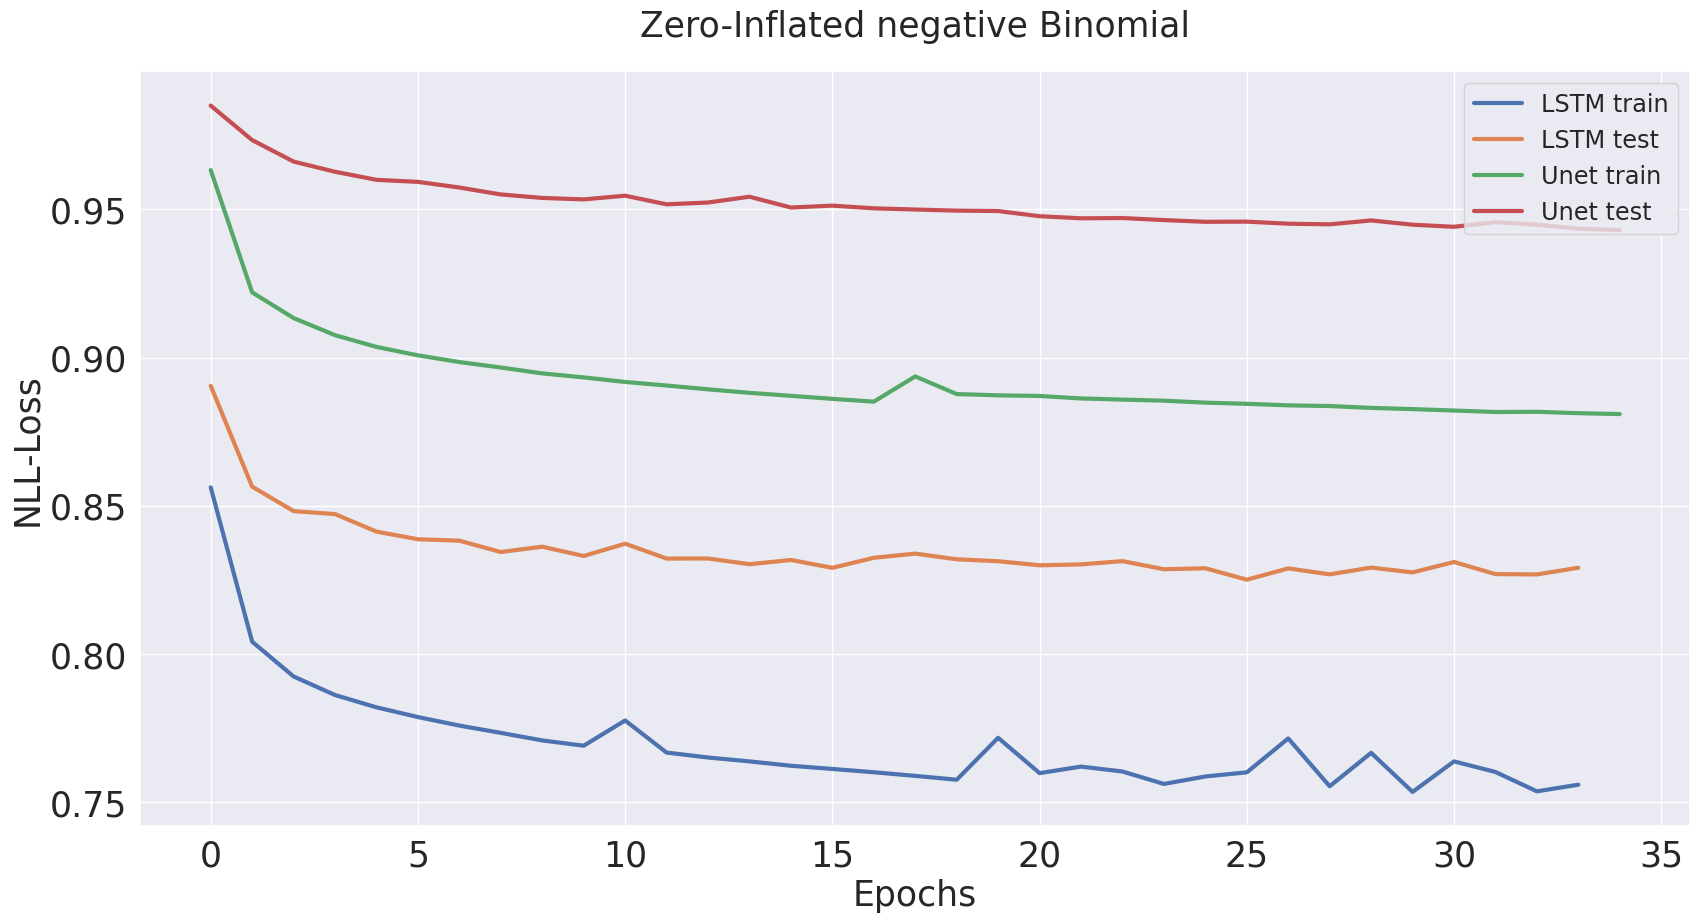
\includegraphics[width=0.9\textwidth,angle=0]{abb/Loss_zinfBinom.png}
 \caption{Trainingskurven für ZINB}
\label{fig:Inception-Conv-LSTM}
\end{figure}

\noindent Zu sehen ist, dass die Unet-Architektur schlechtere Performance als die LSTM-Architektur liefert. In dieser Abbildung scheint der Overfitting bereich noch nicht erreicht worden zu sein.
Tatsächlich verbessern sich beide Architekturen noch marginal nach weiteren Epochen, aus Darstellungsgründen wurde die X-Achse auf 35 Epochen beschnitten.\\

\noindent Zusätzlich zur ZINB wurden beide Architekturen mit einer weiteren Verteilung trainiert. Hierfür verwenden wir die Multinomiale Verteilung, woebei wir die Daten in Sieben Klassen einteilen. Die geschieht durch logarithmisches skalieren der Daten. Dadurch soll zusätzlich dem Klassenungleichgewicht entgegengesteuert werden (Regenwerte im höheren Bereich kommen seltener vor). 

\begin{figure}[htb]
 \centering
 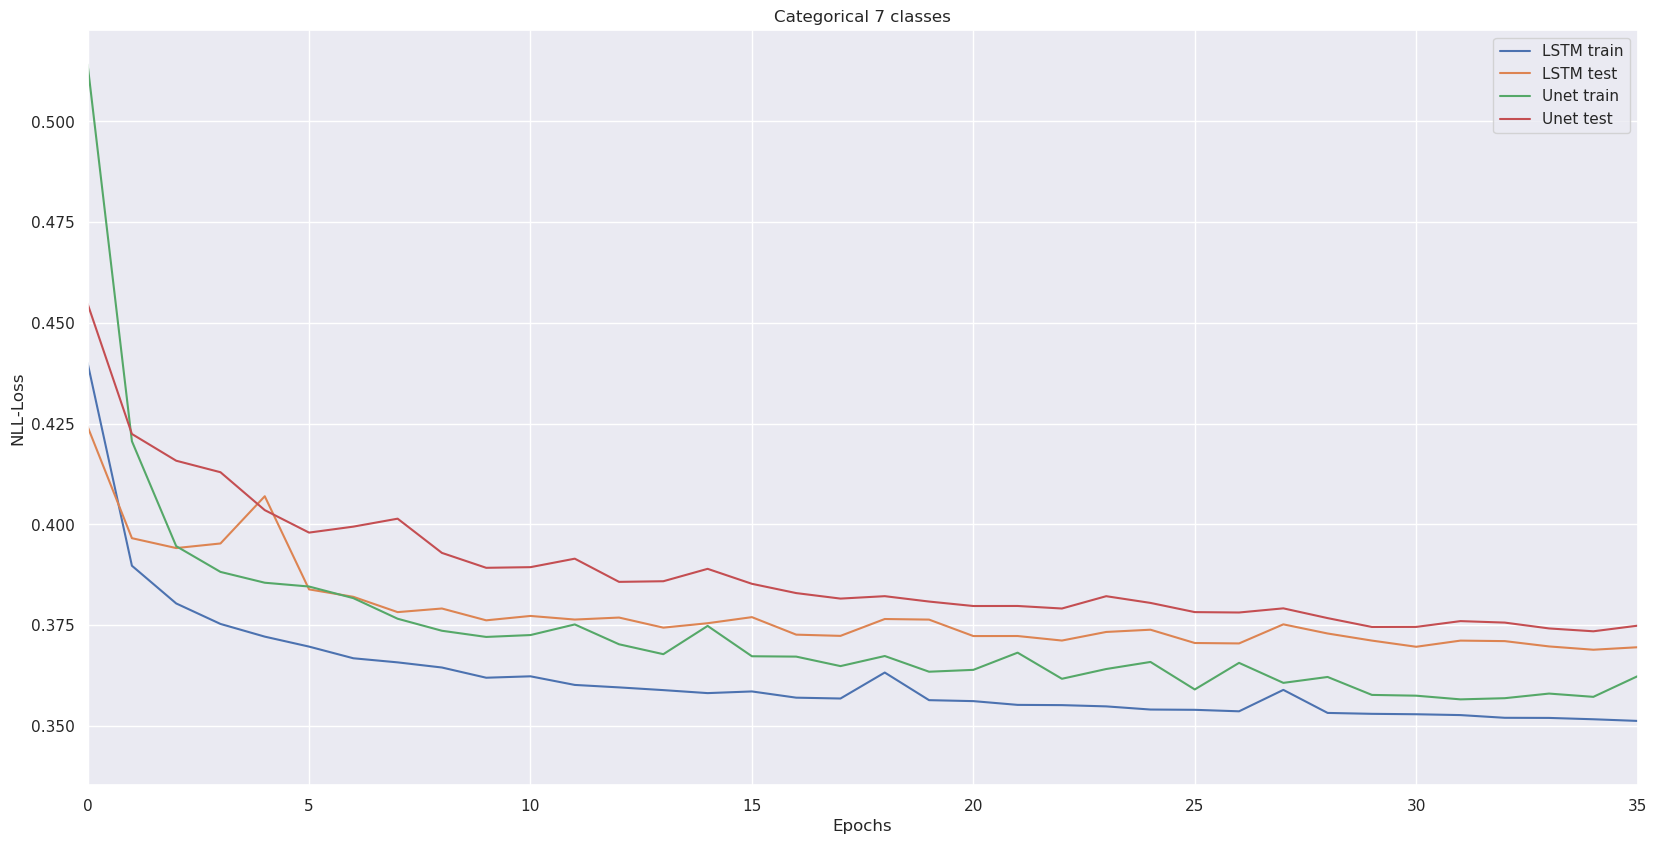
\includegraphics[width=0.9\textwidth,angle=0]{abb/Categorical.png}
 \caption{Multinomiale Verteilung}
\label{fig:multinomialeVerteilung}
\end{figure}

\noindent In der obigen Abbildung sind die Trainingskurven der beiden Architekturen zu sehen. Auch hier ist zu sehen, dass die LSTM-Architektur der Unet-Architektur überlegen ist und dies eine bessere Performance liefert. Vergleicht man die Trainingskurven für beide Verteilungen sieht man, dass der NLL für die Multinomiale Verteilung etwa die Hälfte der ZINB entspricht.

\newpage
\subsection{Auswertung}

Wir beschränken uns zuerst auf die Auswertung der binären Klassifikation von Regen und kein Regen. Später werden wir für die verschiedenen Architekturen und Verteilungen die Klassifikation für die Regenvorhersage begutachten.

%\subsubsection{Baseline}
%TODO:

\subsubsection{Auswertung der binären Regenvorhersage}
Die folgende Abbildung zeigt einen zufälligen Ausschnitt der Regenvorhersage für sieben aufeinanderfolgende Zeitschritte.\\

\begin{figure}[h]
\begin{tabular}{lllllll}
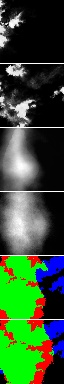
\includegraphics[width=20mm]{abb/prediction/100_maxCont}&
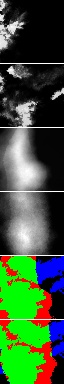
\includegraphics[width=20mm]{abb/prediction/101_maxCont}&
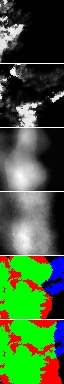
\includegraphics[width=20mm]{abb/prediction/102_maxCont}&
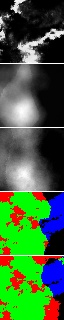
\includegraphics[width=20mm]{abb/prediction/103_maxCont}&
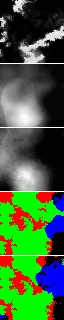
\includegraphics[width=20mm]{abb/prediction/104_maxCont}&
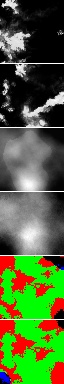
\includegraphics[width=20mm]{abb/prediction/105_maxCont}&
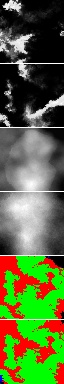
\includegraphics[width=20mm]{abb/prediction/106_maxCont}
\end{tabular}
\caption{Vorhersage in Abständen von fünf Minuten für die ZINB. Die erste Zeile entspricht dem momentanen Regen. Zeile zwei entspricht dem tatsächlichen Regen in 30 Minuten. Zeile drei ist die 30 Minuten Vorhersage des Unets. Zeile vier ist die 30 Minuten Vorhersage der LSTM-Architektur. Für die Vorhersage wurde der Mittelwert der Verteilung berechnet. Die Bilder sind kontrastmaximiert dargestellt. Die letzten beiden Zeilen stellen die korrekte bzw. inkorrekte Regenvorhersage für die Unet- und die LSTM-Architektur (letzte Zeile) dar.
Hierbei entspricht true positiv der Farbe Grün, false positiv Rot, false negativ Blau und true negativ Schwarz .\label{fig:predNegBin}}
\end{figure}

\noindent Anhand der Abbildung \ref{fig:predNegBin} ist zu sehen, dass für beide Architekturen tendenziell zu viel Regen vorhergesagt wird. Anhand der Bilder ist zudem zu sehen, dass Form der Regenfront nicht korrekt vorhergesagt wird. Des weiteren ist zu erkennen, dass false negativ (Blau) einen geringeren Teil der Vorhersage ausmachen. Durch die Kontrastmaximierte Darstellung der Vorhersage, sehen die Bilder so aus, als würden die maximalen Werte der Vorhersage in etwa der maximalen Werte des tatsächlichen Wetters entsprechen. Tatsächlich wird im allgemeinen die Regenmenge unterschätzt. Dies wird in einem späteren Teil der Auswertung dargelegt.\\



\begin{figure}[h]
\begin{tabular}{lllllll}
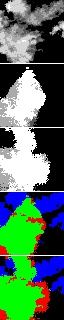
\includegraphics[width=20mm]{abb/prediction/100_cat_maxCont}&
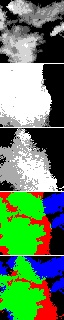
\includegraphics[width=20mm]{abb/prediction/101_cat_maxCont}&
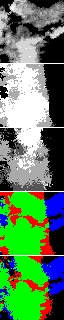
\includegraphics[width=20mm]{abb/prediction/102_cat_maxCont}&
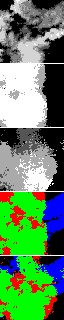
\includegraphics[width=20mm]{abb/prediction/103_cat_maxCont}&
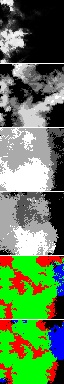
\includegraphics[width=20mm]{abb/prediction/104_cat_maxCont}&
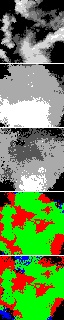
\includegraphics[width=20mm]{abb/prediction/105_cat_maxCont}&
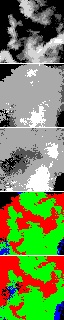
\includegraphics[width=20mm]{abb/prediction/106_cat_maxCont}
\end{tabular}
\caption{Vorhersage in Abständen von fünf Minuten für die Multinomialverteilung. Hier sind die Zeilen wie in \ref{fig:predNegBin} dargestellt. Alle Bilder bis auf die Bilder der ersten Zeile sind in sieben Klassen dargestellt.\label{fig:predCat}}
\end{figure}


\noindent Auch bei der Multinomialenverteilung wird tendenziell zu viel Regen vorhergesagt. Für die Vorhersage wird das Label mit der größten Wahrscheinlichkeit herangezogen. Es ist erkennbar, dass die Form der Regenfront nicht korrekt vorhergesagt. Zudem scheint die Anzahl der false negative (Blau) Vorhersagen höher als bei der ZINB. Zusammenfassend ist für die Ausschnitte der Vorhersagen zu sagen, dass die true positive vorhersagen die false negative und false positiv überwiegen. Um eine generelle Aussage treffen zu können wir im weiteren Verlauf die ''receiver operating characteristic'' auch \textbf{ROC} herangezogen.


\noindent In der folgenden Abbildung ist die ROC für beide Architekturen und Verteilungen zu sehen. Die Kurven entstehen indem wir für verschiedene Schwellwerte die binäre Regenvorhersage treffen. Das bedeutet konkret, dass die Wahrscheinlichkeit für kein Regen berechnet wird. Ist diese Wahrscheinlichkeit größer als der Schwellwert so wird auch kein Regen vorhergesagt.
Die Schwellwerte liegen gleichmäßig verteilt zwischen Null und Eins.


\begin{figure}[h]
\begin{tabular}{cc}
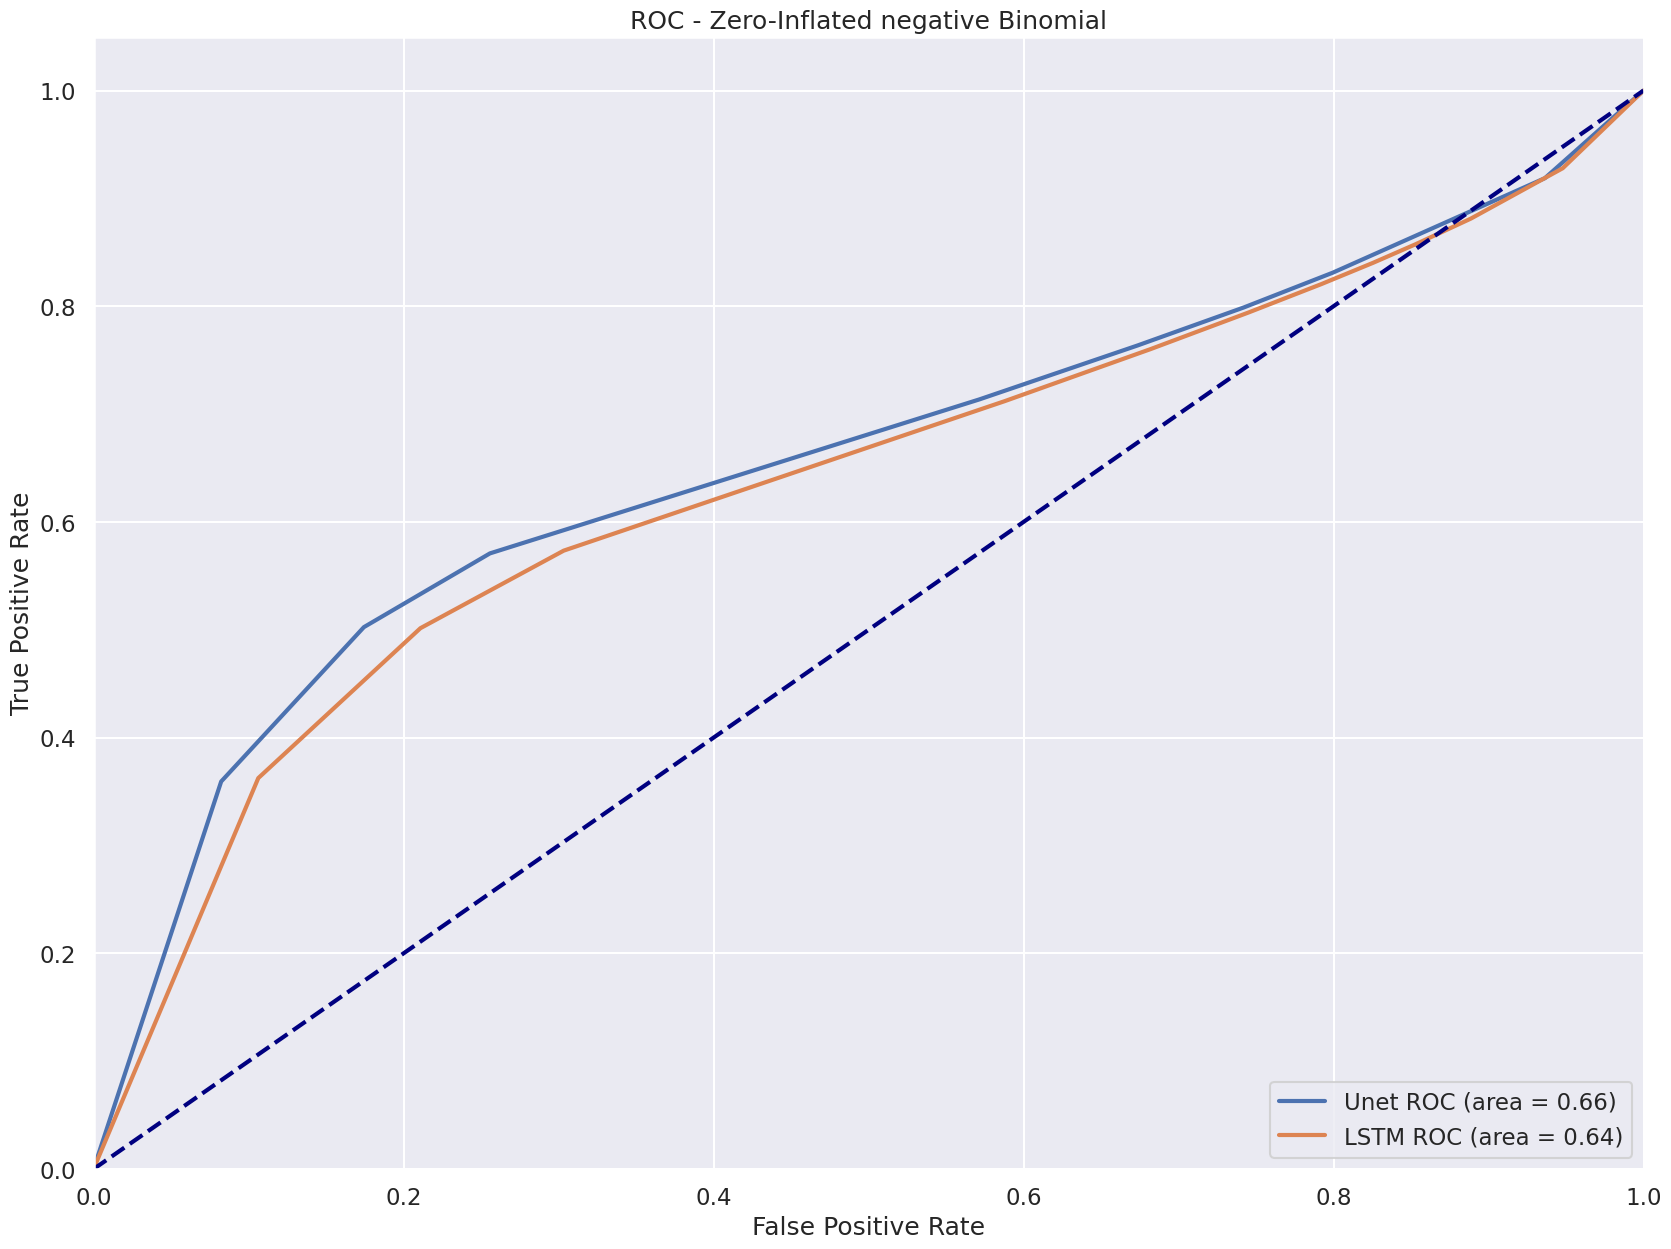
\includegraphics[width=70mm]{abb/ROC_ZINFBINOM.png}&
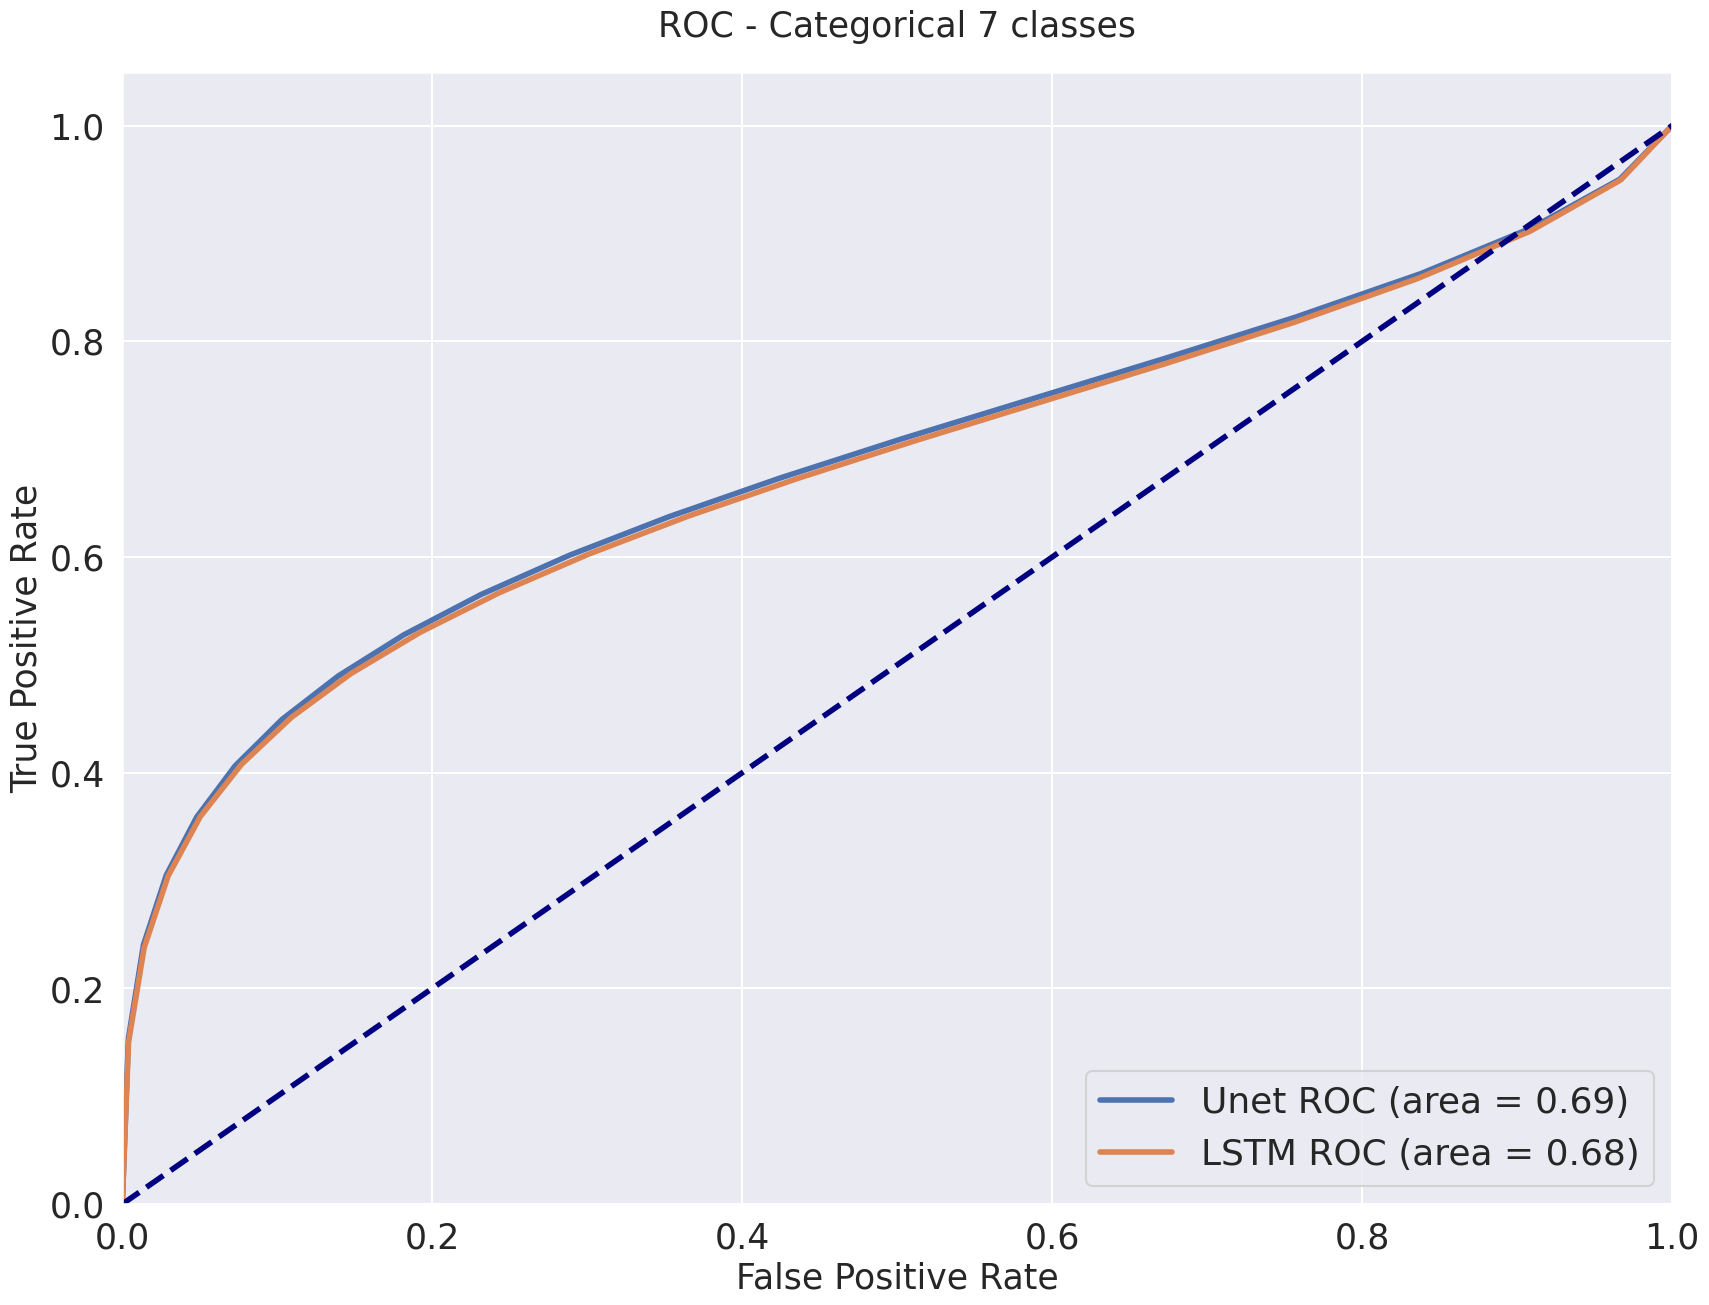
\includegraphics[width=70mm]{abb/ROC_Categorical.png}
\end{tabular}
\caption{ROC/AUR für beide Architekturen und beide Verteilungen. Links für die ZINB und rechts für die Multinomialverteilung.
Die Auserwertung erfolgt für 20 verschiedene Schwellwerte. \label{fig:anomerz}}
\end{figure}

\noindent Wie Anhand der Kurven zu erkennen ist, ist die ROC für die Multinomialverteilung gleichmäßiger als die für die ZINB. 
Auch die Fläche unter der Kurve (''area under curve'' \textbf{AUC}) ist für die Multinomialverteilung marginal größer. Interessanterweise ist die Performance des Unets bei beiden Verteilungen besser (auch hier nur marginal) als für die LSTM-Architektur.\\

\noindent Für den Schwellwert 0.5 erhalten wir in beiden Fällen ein relativ gutes Verhältnis von true positiv zu false positiv. In den Nachfolgenden Abbildungen ist die Confusionmatrix für diesen Schwellwert zu sehen.



\begin{figure}[h]
\begin{tabular}{ccc}
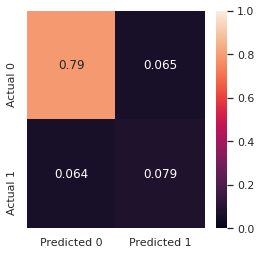
\includegraphics[width=45mm]{abb/simpleBaseLine.png}&
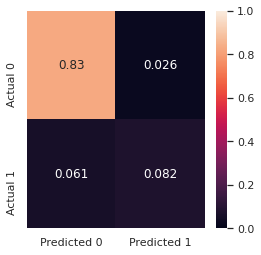
\includegraphics[width=45mm]{abb/znBinomConfusion_LSTM.png}&
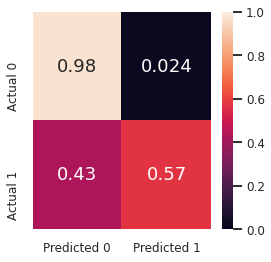
\includegraphics[width=45mm]{abb/znBinomConfusion_UNET.png}
\end{tabular}
\caption{Confusionmatrix für die ZINB und dem Schwellwert 0.5. Links die einfache Baseline, mittig für die LSTM-Architektur und rechts für die Unet-Architektur. \label{fig:confusionmatrix_binom}}
\end{figure}

\noindent Anhand der Confusionmatrix ist zu sehen, dass die Netzwerke in beiden Fällen eine bessere Vorhersage liefern als die einfache Baseline. 
Anhand der Confusionmatrix wird das ungleichgewicht zwischen Regen und kein Regen deutlich. 

\begin{figure}[h]
\begin{tabular}{ccc}
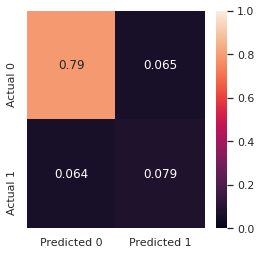
\includegraphics[width=45mm]{abb/simpleBaseLine.png}&
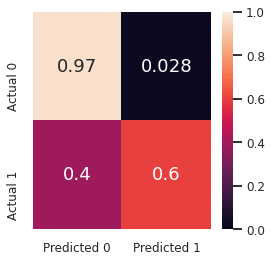
\includegraphics[width=45mm]{abb/categoricalConfusion_LSTM.png}&
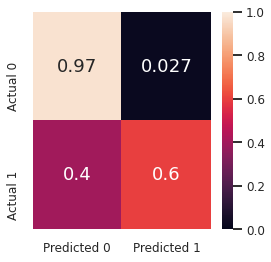
\includegraphics[width=45mm]{abb/categoricalConfusion_UNET.png}
\end{tabular}
\caption{Confusionmatrix für die Multinomialverteilung und dem Schwellwert 0.5. Links die einfache Baseline, mittig für die LSTM-Architektur und rechts für die Unet-Architektur. \label{fig:confusionmatrix_cat}}
\end{figure}

\noindent Auch für die Multinomialverteilung erhalten wir eine bessere Vorhersage als mit der einfachen Baseline.
Vergleichen wir die Confusionmatrix beider Verteilungen, so lässt sich feststellen, dass die Verteilungen in verschiedenen Bereichen andere Vorteile aufweisen.
So ist die Regenvorhersage für die Multinomialverteilung etwas besser als für die ZINB. Letztere (insbesondere die Unet-Variante) produziert mehr true negative und weniger false positiv Vorhersagen als die Multinomialverteilung.\\

\noindent Für die tatsächliche Regenvorhersage ist jedoch interessant, in wie vielen Fällen eine Person Nass wird obwohl kein Regen vorhergesagt wird.
Dazu wird die untere Zeile der Confusionmatrix mit einem Faktor multipliziert, sodass deren Summe 100 ergibt.\\
\begin{table}[h]
\begin{tabular}[h]{l|c|c}
Verteilung & Person wird Nass & Person wird nicht Nass  \\
\hline
Multinomialverteilung & \textbf{39,9} \% & \textbf{60,1} \%  \\
ZINB &43,0 \% & 57,0 \%  \\
Einfache Baseline & 44,8 \% & 55,2 \% 
\end{tabular}
\caption{Wahrscheinlichkeit trocken zu bleiben\label{tab:nass}}
\end{table}

\noindent Aus der Tabelle \ref{tab:nass} hervorgeht, wird die Person die sich auf die Vorhersage verlässt mit einer Wahrscheinlichkeit von 39,1 (im besten Fall) \% Nass.
Dies ist zwar nicht überragend, es ist jedoch besser als würde sich die Person darauf verlassen, dass das Wetter so bleibt wie es ist.

\newpage
\subsubsection{Auswertung der Regenvorhersage}
\noindent Ein weiterer interessanter Aspekt ist die Genauigkeit der Vorhersage für den Regenfall. Hierfür betrachten wir zuerst die ZINB.
Hierfür berechnen wir das Konfidenzintervall der Verteilung welches 97,5\% der Daten umschließt. Daraufhin zählen wir wie oft der wahre Wert innerhalb des Konfidenzintervalls liegt.
In der folgenden Abbildung sind die zwei 97,5 \% Konfidenzintervalle für die beiden Architekturen zu sehen.\\

\begin{figure}[h]
\centering
\begin{tabular}{c}
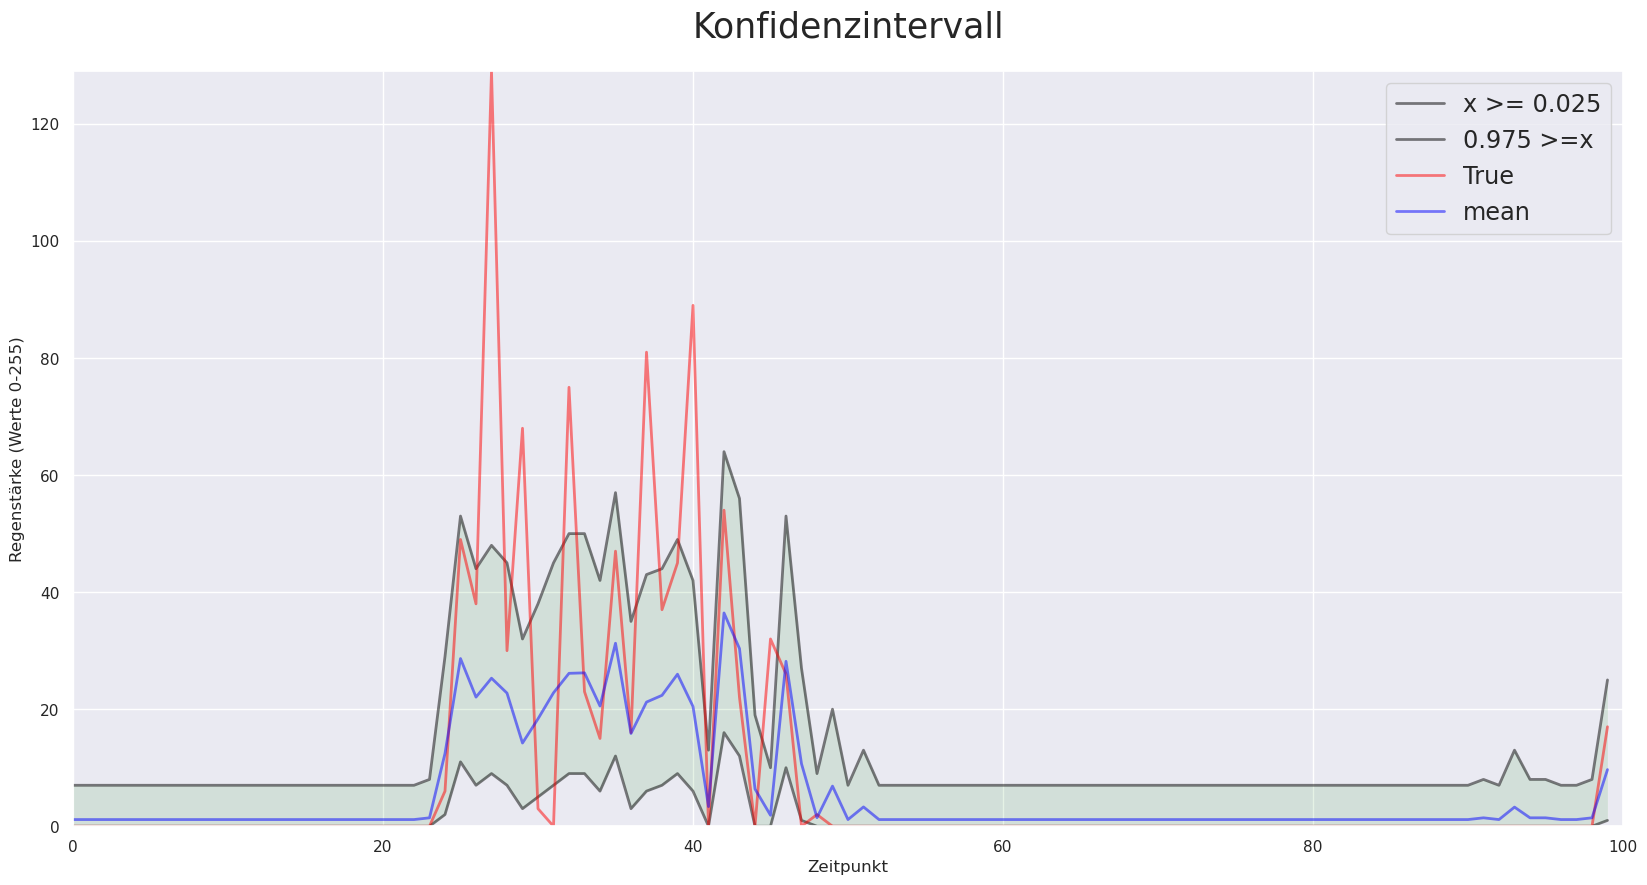
\includegraphics[width=120mm]{abb/quantile_LSTM.png}\\
(a) \small{LSTM-Architektur}\\
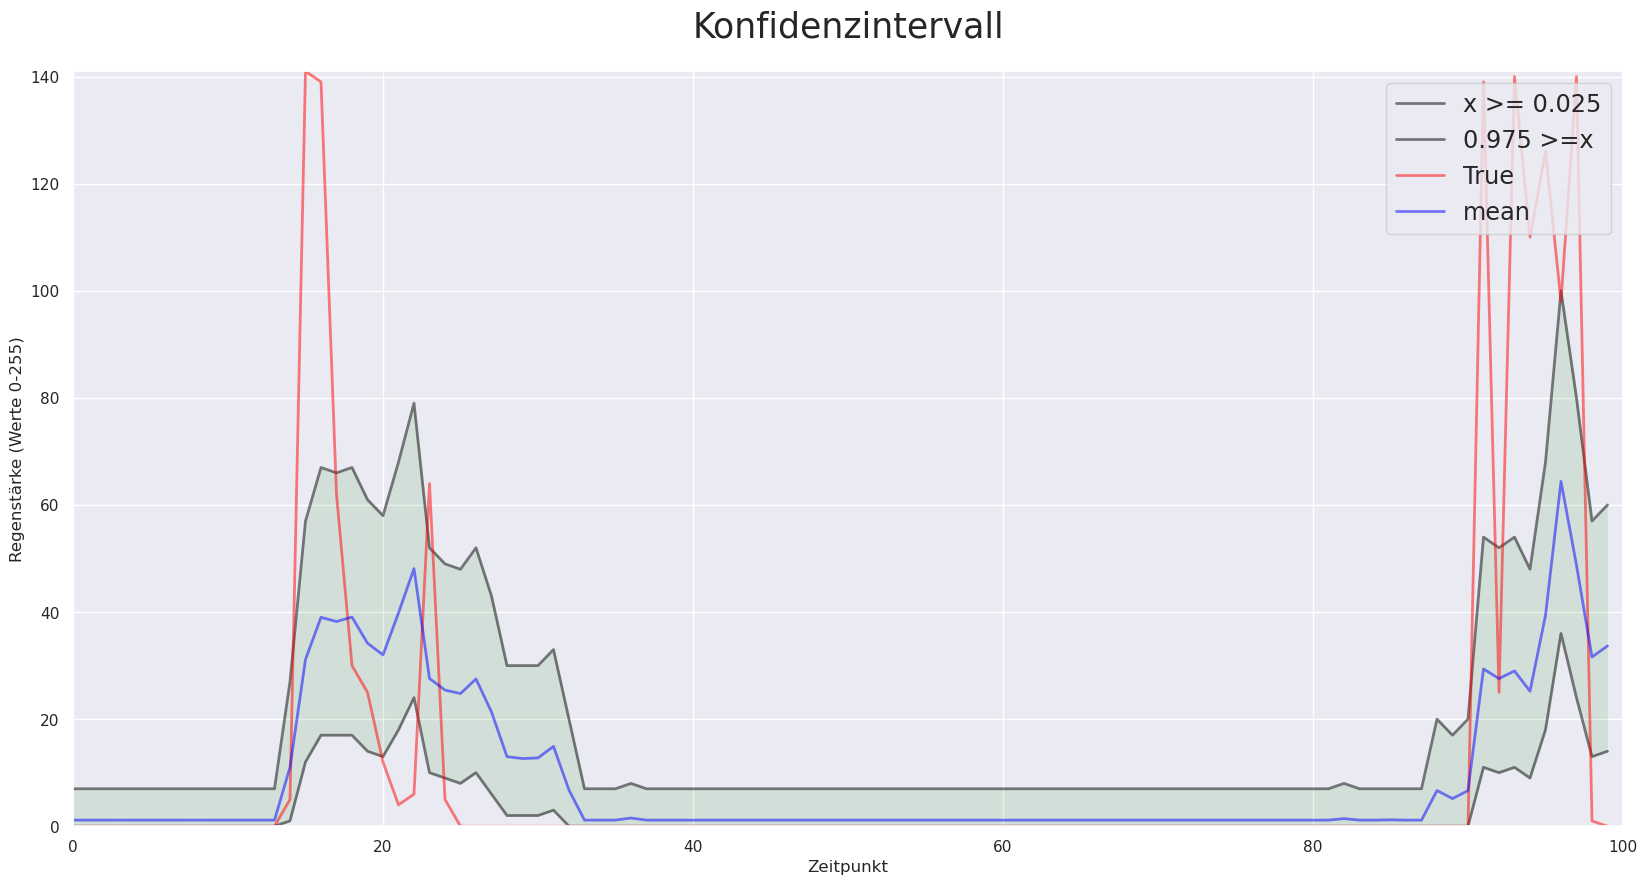
\includegraphics[width=120mm]{abb/quantile_UNET.png}\\
(b) \small{UNET}
\end{tabular}
\caption{Konfidenzintervall für die ZINB, Oben für die LSTM-Architektur, unten für das UNET. \label{fig:konfidenzintervall}}
\end{figure}

\noindent Die Konfidenzintervalle sind hierbei über eine Sequenz eines zufälligen Ausschnitts eines Pixels berechnet. Sie sind deshalb nicht aussagekräftig für die Vorhersage, sondern sollen lediglich die Erklärung für das Vorgehen vereinfachen. Anhand der Abbildungen ist zu sehen, dass die Konfidenzintervalle in etwa dem ''wahren'' Wert folgen. Allerdings ist auch zu sehen, dass Extremwerte meist außerhalb des Intervalls liegen. Zählen wir nun die Anzahl der Vorhersagen, bei denen der wahre Wert im Konfidenzintervall liegt, so ergibt sich folgendes Histogramm.\\


\begin{figure}[h]
\centering
\begin{tabular}{cc}
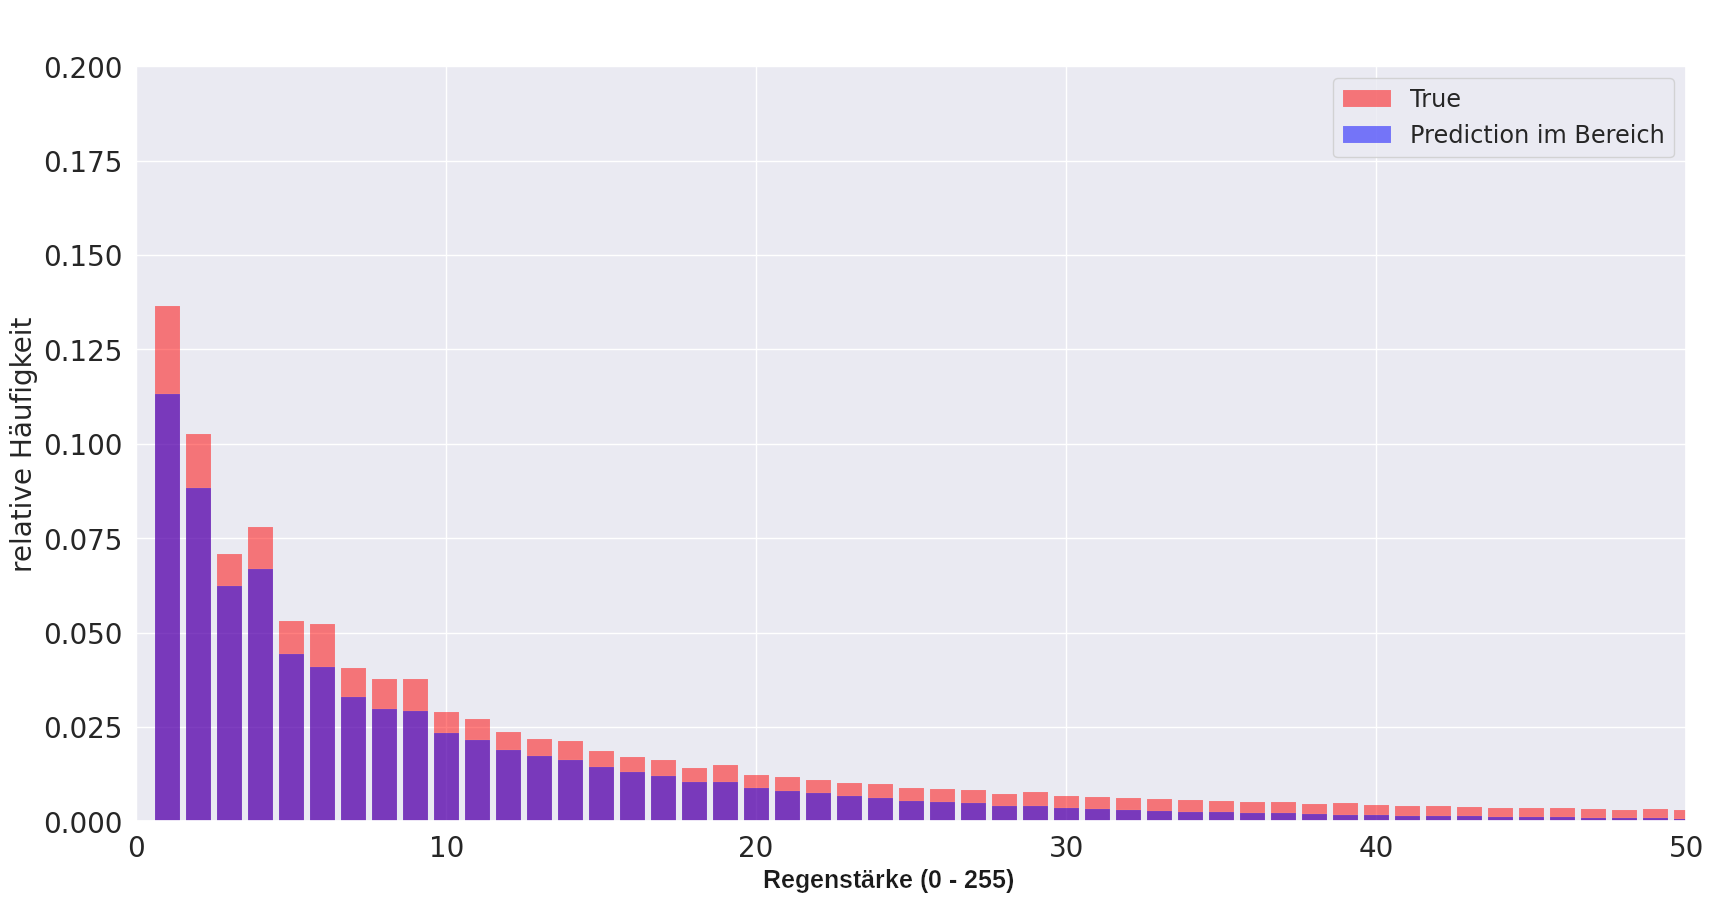
\includegraphics[width=80mm]{abb/dist_LSTM.png}&
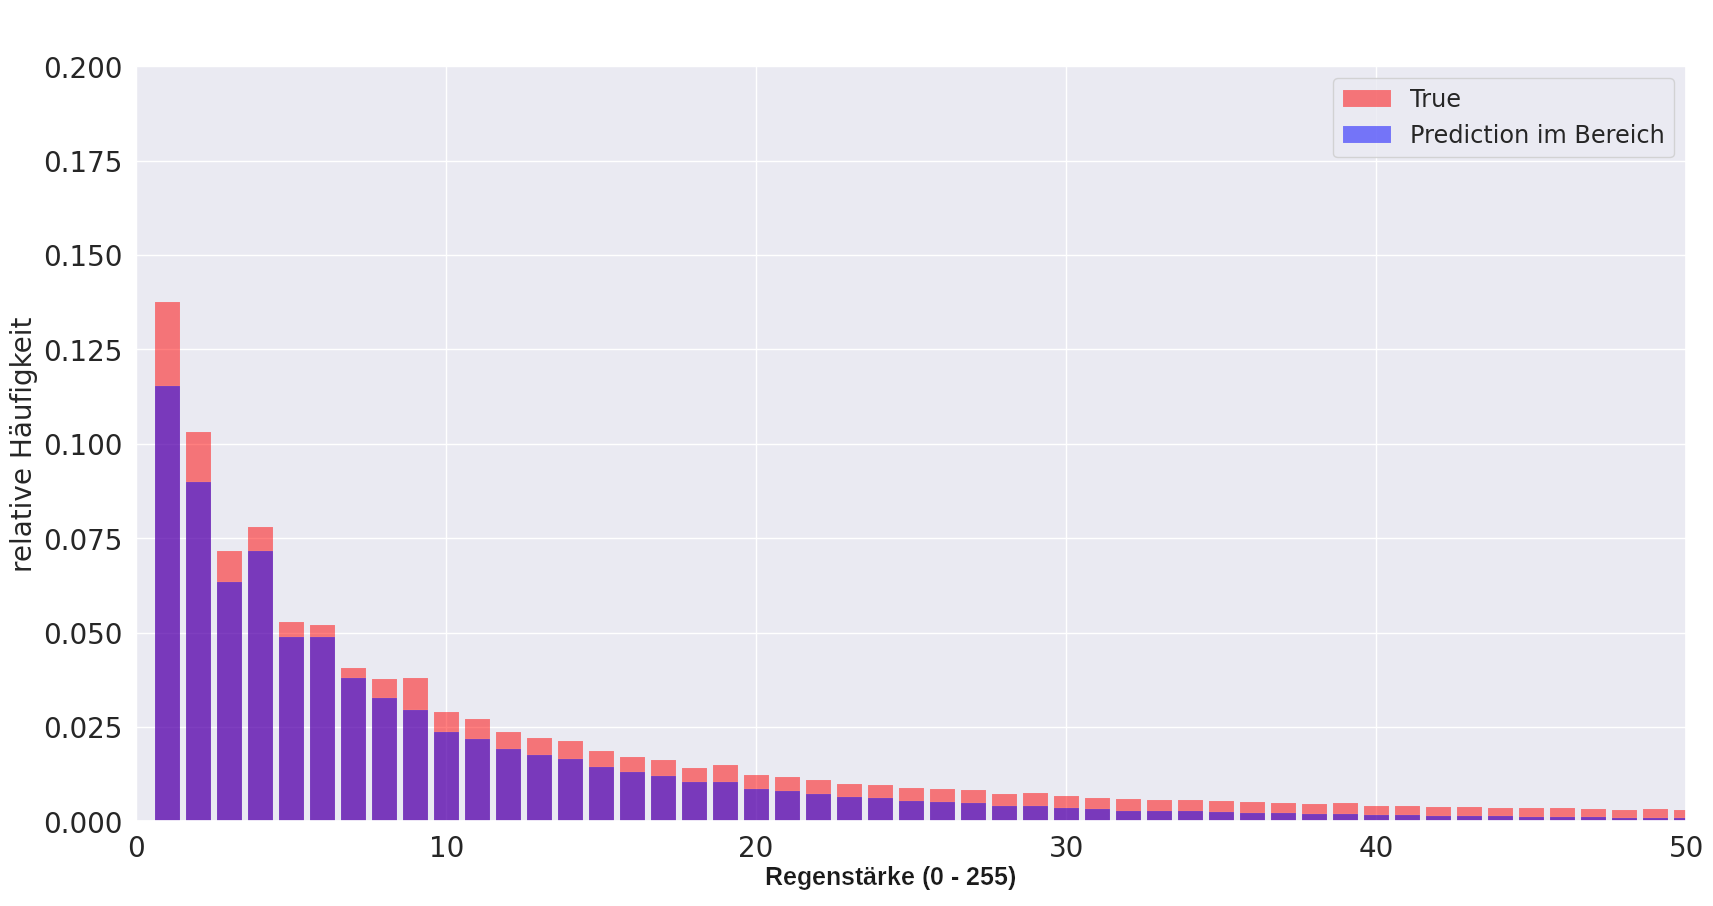
\includegraphics[width=80mm]{abb/dist_UNET.png}\\
(a) \small{LSTM-Architektur} & (b) \small{UNET}
\end{tabular}
\caption{Relative Anzahl der ground truth im Konfidenzintervall. \label{fig:dist}}
\end{figure}

\noindent Anhand der Diagramme ist zu sehen, dass der ''wahre'' Wert in den meisten Fällen von der Verteilung umschlossen wird. Für die Diagramme wurde der Balken der kein Regen repräsentiert weggelassen. Für größere Regenwerte sieht man, dass der ''wahre'' Wert selten innerhalb der Konfidenzintervalle liegt. Daraus folgt, dass die Vorhersage mit der Zunahme der Regenstärke schlechter wird.\\



\begin{table}[h]
\centering
\begin{tabular}[h]{l|c|c|c}
Architektur & inklusive kein Regen & exklusive kein Regen & Konfidenzintervall \\
\hline
UNET & \textbf{93,0} \% & \textbf{73,0} \%  & 97,5 \%\\
 & 88,0 \% & 43,0 \% & 95 \% \\
 & 86,0 \% & 35,0 \% & 90 \% \\
 \hline
LSTM &92,0 \% & 71,0 \% & 97,5 \% \\
 &\textbf{89,0} \% & \textbf{45,0} \% & 95 \% \\
 &\textbf{87,0} \% & \textbf{40,0} \% & 90 \% \\

\end{tabular}
\caption{ Relative Anzahl der wahren Werte im Konfidenzintervall für verschiedene Intervalle und Architekturen\label{tab:konv}}
\end{table}

\noindent In Tabelle \ref{tab:konv} ist zu erkennen, dass je kleiner das Konfidenzintervall gewählt wird, desto seltener liegt die ground truth im Konvidenzintervall.
Für die Spalte ''inklusive Regen'' ist der Unterschied nur marginal. Für die Spalte ''exklusive kein Regen'' ist ein großer Sprung zwischen dem 97,5 \% und dem 95 \% Konvidenzintervall zu sehen.
Dies kann so interpretiert werden, dass die ground truth für diese Fälle nicht im ''Zentrum'' des Konfidenzintervalls liegt (bzw. weiter entfernt vom Zentrum). Der Mittelwert ist für diese Fälle eine schlechte Schätzung für die ground truth.\\

\noindent Schauen wir uns nun die Multinomialverteilung an. Wir gehen ähnlich vor wie bei der ZINB vor und stellen die Anzahl der korrekten Vorhersagen gegenüber der Anzahl der ground truth (pro label). Um dies mit der ZINB vergleichen zu können, skalieren wir die Vorhersage der ZINB logarithmisch und stellen dies ebenfalls als Histogramm dar. Die folgende Abbildung zeigt das Ergebnis dieser Vorgehensweise.\\

\begin{figure}[h]
\centering
\begin{tabular}{c|c}
\small{LSTM} & \small{UNET}\\
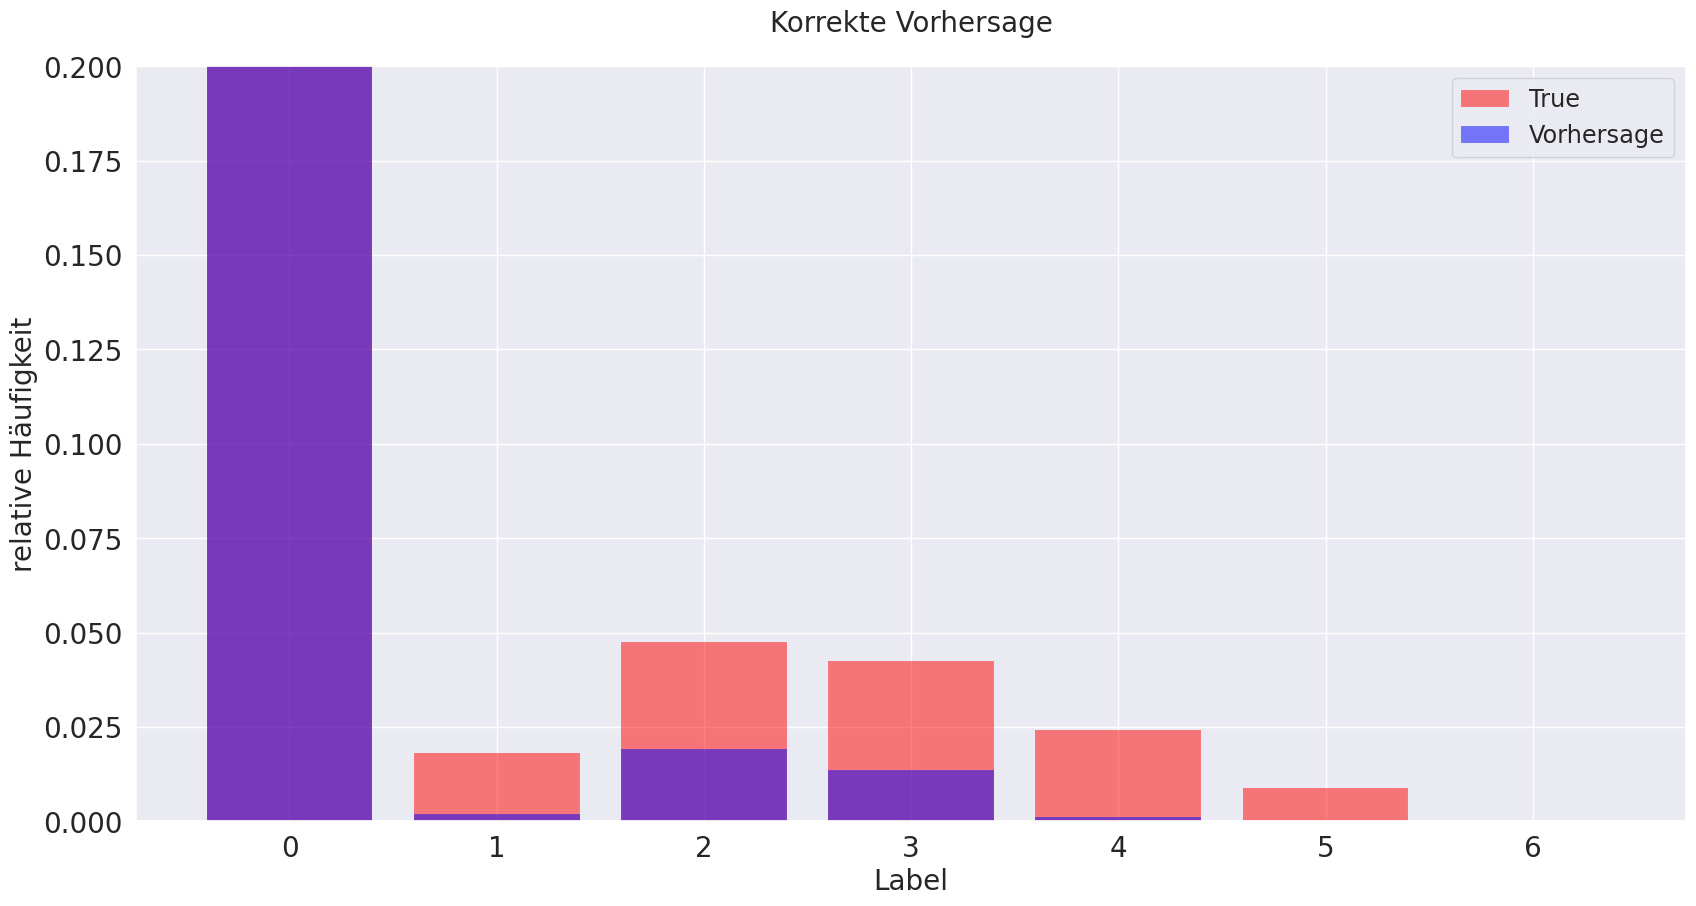
\includegraphics[width=80mm]{abb/LSTM_LOGBIN.png}&
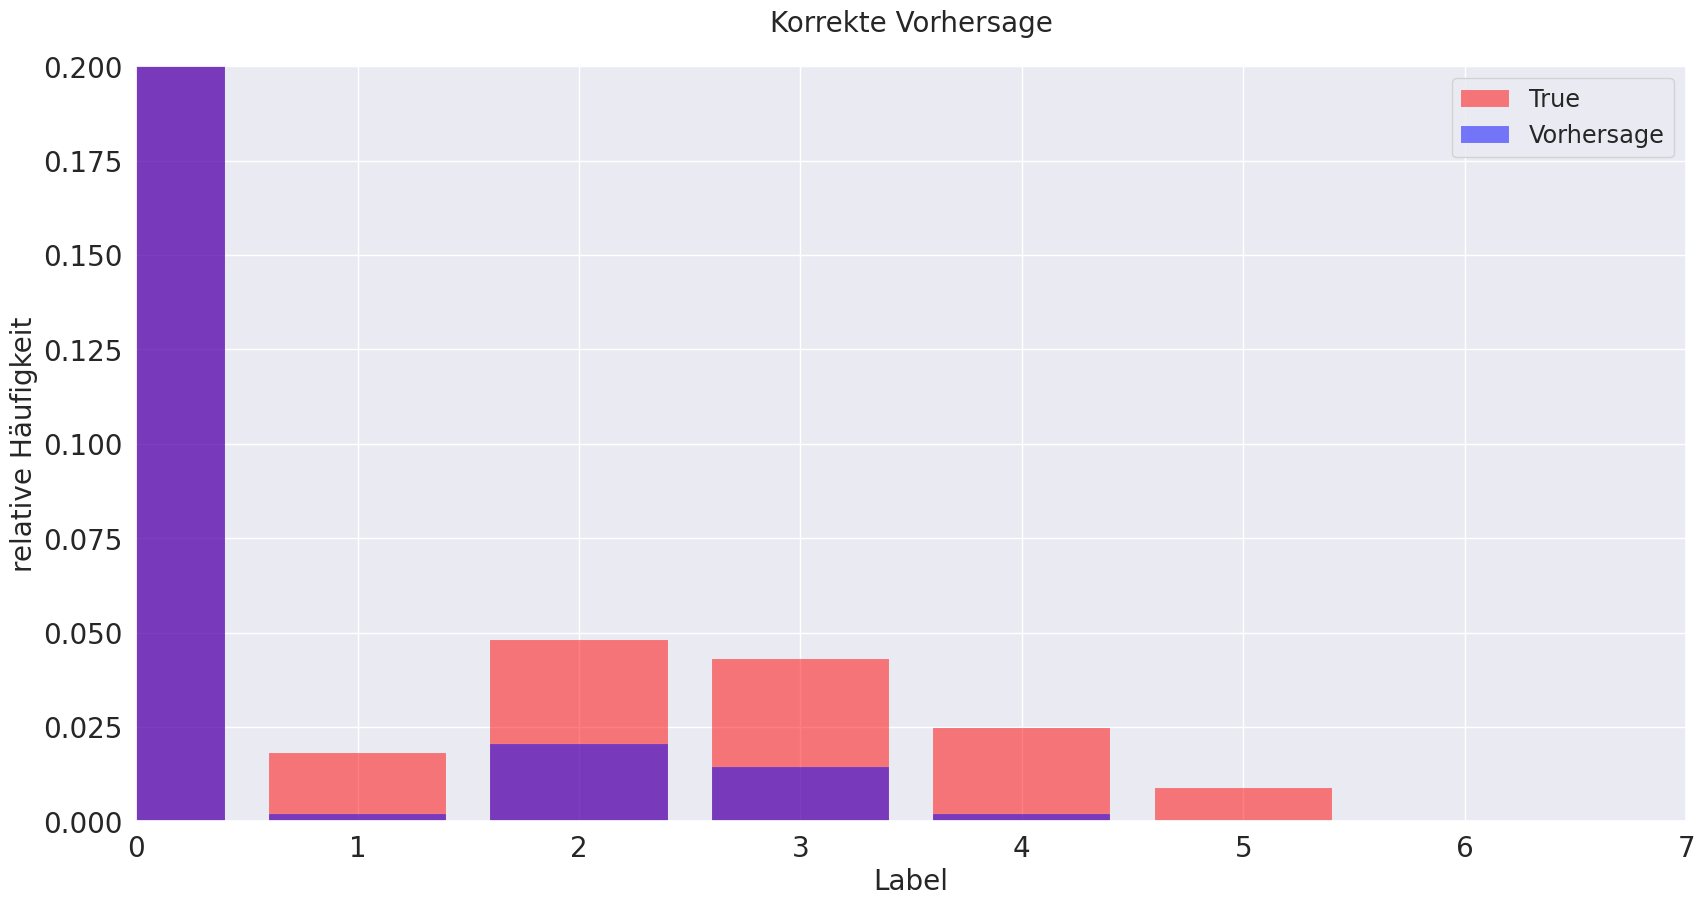
\includegraphics[width=80mm]{abb/UNET_LOGBIN.png}\\
\hline
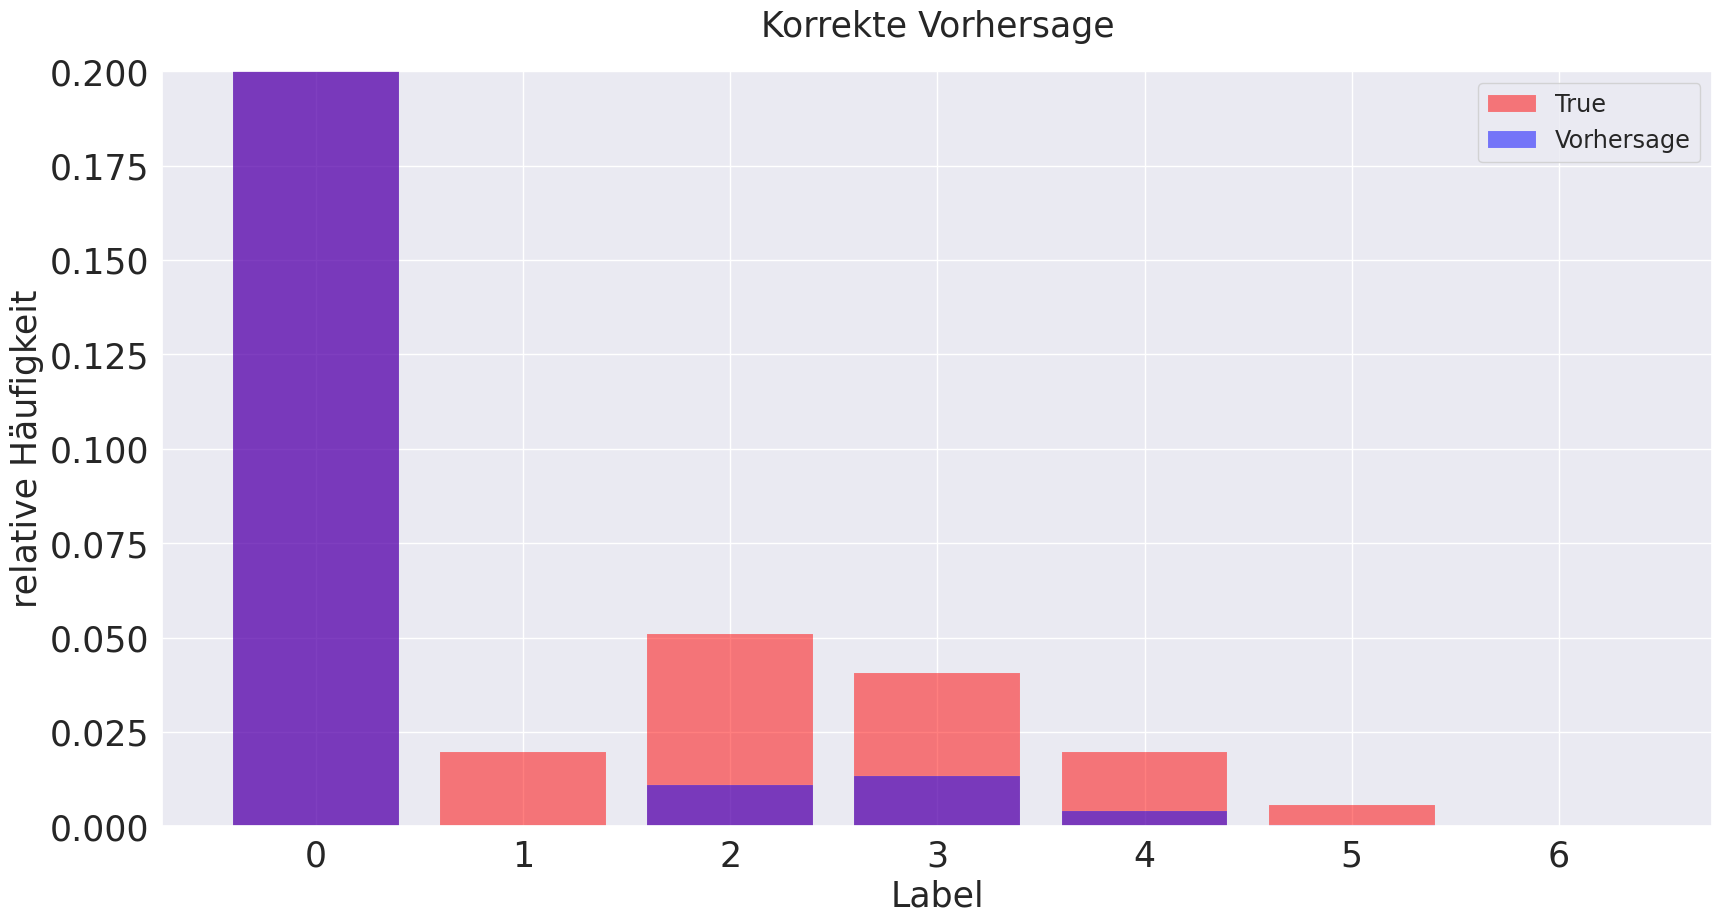
\includegraphics[width=80mm]{abb/dist_cat_lstm.png}&
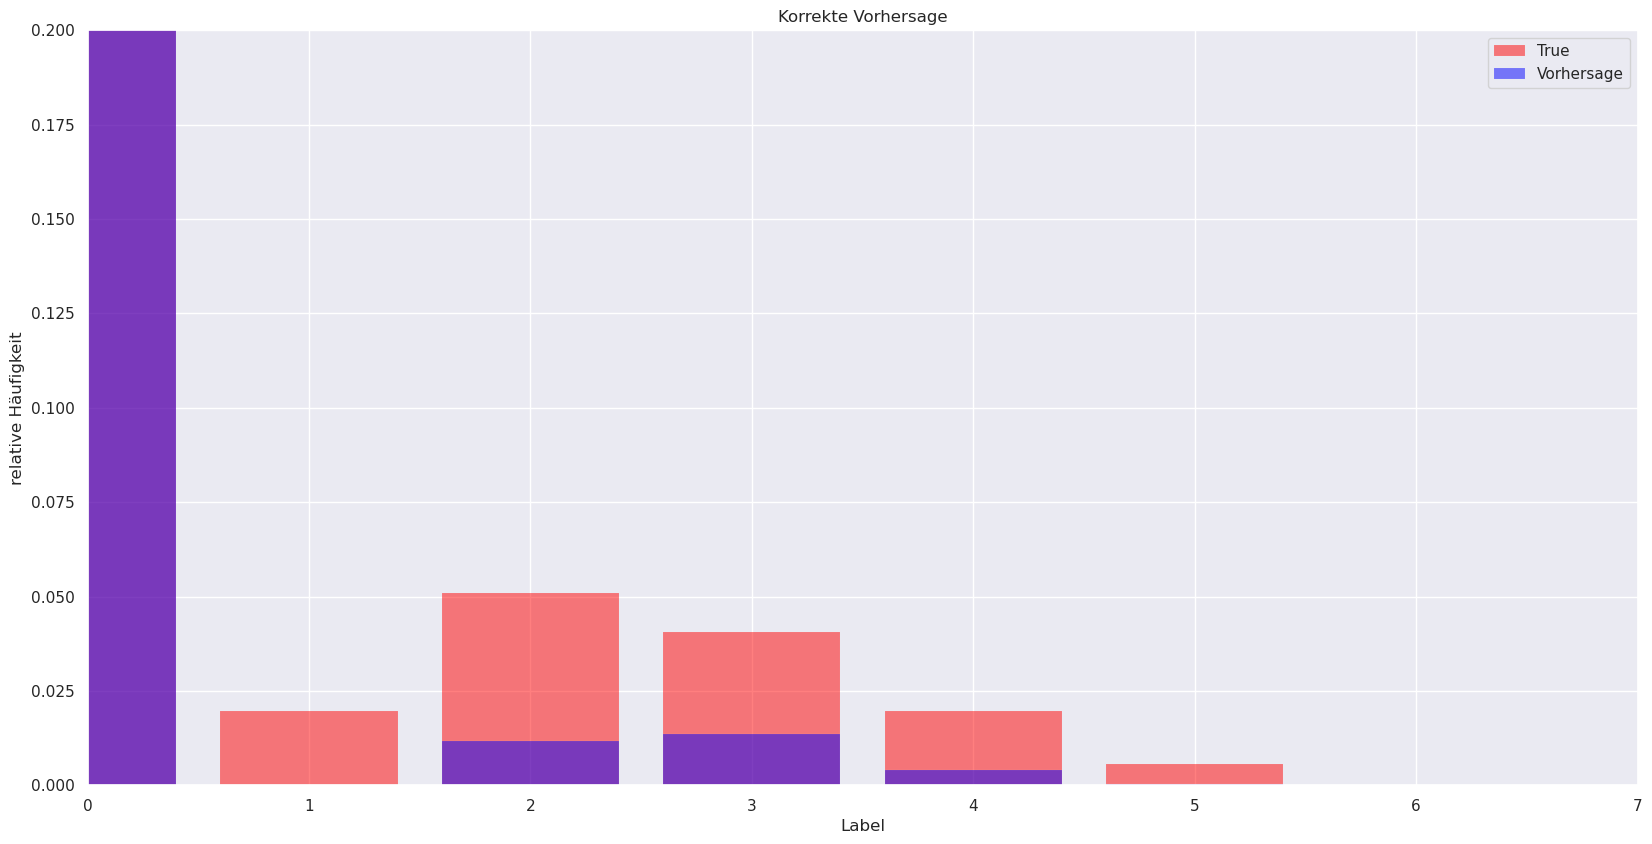
\includegraphics[width=80mm]{abb/dist_cat_unet.png}\\
\end{tabular}
\caption{Histogramm der Vorhersagen für beide Verteilungen und Architekturen. Die erste Zeile entspricht der ZINB, die letzte der Multinomialverteilung \label{fig:logDist}}
\end{figure}

\noindent Anhand des Histogramms ist zu erkennen, dass die ZINB eine leicht bessere Vorhersage liefert. Das Histogramm wurde in Richtung y-achse bei 0.2 begrenzt um eine bessere Darstellung zu erreichen. Stellt man die Beziehung in einer Tabelle dar, so kommt man zu folgendem Ergebnis.\\

\begin{table}[h]
\centering
\begin{tabular}[h]{|l|c|c|c|c|}
\hline
&\multicolumn{2}{c}{exklusive kein Regen} &
\multicolumn{2}{c|}{inklusive kein Regen} \\
\hline
& LSTM & UNET & LSTM & UNET \\
\hline
ZINB & 26 \% & 27 \% & 78 \% & 78 \% \\
Multinom & 21 \% & 22 \% & 88 \% & 88 \% \\
\hline
\end{tabular}
\caption{Relative Anzahl der korrekt vorhergesagten Regenwerte\label{tab:raintable}}
\end{table}

\noindent Anhand der Tabelle \ref{tab:raintable} ist ersichtlich, dass die ZINB eine bessere Vorhersage für die Regenstärke liefert. Die Multinomialverteilung hingegen liefert eine bessere Vorhersage im allgemeinen.

\subsubsection{Fazit der Auswertung}

Für die binäre Regenvorhersage ist Multinomialverteilung die Verteilung welche die besten Resultate liefert. Laut Tabelle \ref{tab:nass} bleibt eine Person zu 60,1 \% trocken, wenn sie sich auf die Vorhersage verlässt. Hierbei spielt es keine Rolle ob die UNET oder die LSTM-Architektur verwendet wird. Da der Loss für die LSTM-Architektur besser als für die Unet-Architektur ist(siehe Abbildung \ref{fig:multinomialeVerteilung}), bevorzugen wir hier die LSTM-Architektur. Für die Klassifikation der Regenvorhersage liefert die Verteilung der ZINB die besten Resultate (siehe Tabelle \ref{tab:raintable}). Hier ist laut Tabelle \ref{tab:raintable} die Unet-Architektur marginal besser. Jedoch ist der Loss der LSTM-Architektur besser (siehe Abbildung \ref{fig:Inception-Conv-LSTM}). Zudem liegt laut Tabelle \ref{tab:konv} die ground truth für kleinere Konfidenzintervalle öfters in eben diesen Intervallen. Daraus schließen wir, dass der Mittelwert näher an der ground truth liegt und dieser dadurch eine bessere Vorhersage liefert. Für unsere Vorhersage wäre es optimal, wenn wir für die binäre Regenvorhersage die Multinomialverteilung und für die Regenklassifikation die ZINB in Kombination mit der LSTM-Architektur verwenden. Da dies nicht praktisch ist verwenden wir für die Vorhersage die LSTM-Architektur mit der ZINB.


